

\documentclass[jou]{apa}%can be jou (for journal), man (manuscript) or doc (document)
%
%
% Bibliography
\usepackage{apacite}
\usepackage{float}
\usepackage[export]{adjustbox}
\usepackage[english]{babel}
\usepackage[latin1]{inputenc}
%these next packages extend the apa class to allow for including statistical and graphic commands
\usepackage{url}   %this allows us to cite URLs in the text
\usepackage{hyperref}

%\usepackage[labelformat=parens,labelsep=quad,skip=3pt]{caption}
\usepackage{graphicx}  %allows for graphic to float when doing jou or doc style
%\usepackage[demo]{graphicx}
\usepackage{caption}
\usepackage{subcaption}
\captionsetup{compatibility=false} 
\usepackage{amssymb}  %use formatting tools  for math symbols
% type setting of functions, packages, and R follows a particular style
\let\proglang=\textsf
\newcommand{\R}{\proglang{R}}
\newcommand{\pkg}[1]{{\normalfont\fontseries{b}\selectfont #1}}
\newcommand{\Rfunction}[1]{{\texttt{#1}}} 
\newcommand{\fun}[1]{{\texttt{#1}}} 
\newcommand{\Robject}[1]{{\texttt{#1}}} 
%
%
%Here is where we start the important APA stuff

\title{Classification for Arctic Cloud Data}
\author{Xuanfu Lu, H. Ham Huang}
\affiliation{Statistics 154 \\ Project 2}


\begin{document}
\maketitle   
%Although the structure of the paper is by AP, these first few paragraphs are by WR
\section{\textbf{Part I: Data exploration and collection}}
\subsection{a) paper summary}
To study the impact of global warming, one cannot evade a careful examination of the North Pole. Fortunately, MISR, launched by NASA in 1999, has equipped scientists with very detailed and comprehensive meteorological photographs of the North Pole. In order to excavate useful information from these photographs, scientists need a good classification algorithm to separate the clouds from the terrain and because the light reflected from the ice cover resembles the one reflected from the clouds, no algorithm up-to-date can classify with a satisfying accuracy and coverage. This paper takes on the challenge and devises two new algorithms, ELCM and ELCM-QDA, which instead of trying to identify clouds, attempts to identify terrains.\\
\indent The input data for the algorithm comes from the photographs captured by the nine cameras on MISR, each viewing the Earth from different angles. Each photograph is converted into pixels and spited into training and testing sets. All pixels are marked by expert as 'cloud', 'not cloud', or 'unsure'. Then, features are drawn to form the dataset. The dataset contains 11 features: x-coordinate, y-coordinate, expert label, 5 radiance angel, and 3 computed features namely NDAI, SD, and CORR. CORR is the average linear correlation coefficient between MISR view directions and it is low for high altitude clouds. CORR alone could be a good predictor for just non-smooth terrain and high altitude clouds. SD is the standard deviation within groups of MISR which is low for smooth terrain. NDAI is the average radiation measurements which is large for low altitude clouds. SD and NDAI together help increase CORR's accuracy on smooth terrain and low altitude clouds. These 3 computed features is pivotal in ELCM's classification. 			The result of this algorithm demonstrates high accuracy and wide coverage. The implication is profound not only for this particular project, but in general for statistical applications in environmental science. It shows that statisticians can play essential role not only in post hoc data analytics, but also directly in processing the raw data to generate predictions and in general, the power of statistics in sciences.

\subsection{b) data summary}
As explained in the paper summary, the data consists of three images shot by MISR from the space: image 1, image 2, and image 3. Each image consists for pixels labeled by experts. '1' means that pixel belongs to the cloudy region, '-1' means clear (terrain) region, and 0 means the expert is unsure (unlabeled). The following summary presents the percentage of each type of pixels: 
\begin{verbatim}
       clear    cloudy   unlabeled
image1 "43.78%" "17.77%" "38.46%" 
image2 "37.25%" "34.11%" "28.64%" 
image3 "29.29%" "18.44%" "52.27%" 
total  "36.78%" "23.43%" "39.79%" 

               clear    cloudy  
image1_labeled "71.13%" "28.87%"
image2_labeled "52.20%" "47.80%"
image3_labeled "61.37%" "38.63%"
total_labeled  "61.08%" "38.92%"
\end{verbatim}
In addition to the expert labeling, the dataset, in which each row represents a pixel, also contains other information (presented as columns): x and y coordinate for each pixel, radiance angel DF, CF, BF, AF, AN, and the computed feature CORR, NDAI, and SD. A summary for 3 images combined:
\begin{verbatim}
    y               x             expert       
 Min.   :  2.0   Min.   : 65.0   Min.   :-1.0000  
 1st Qu.: 98.0   1st Qu.:143.0   1st Qu.:-1.0000  
 Median :193.0   Median :218.0   Median : 0.0000  
 Mean   :193.1   Mean   :218.1   Mean   :-0.1334  
 3rd Qu.:289.0   3rd Qu.:294.0   3rd Qu.: 0.0000  
 Max.   :383.0   Max.   :369.0   Max.   : 1.0000  
      NDAI               SD                CORR        
 Min.   :-1.8420   Min.   :  0.1987   Min.   :-0.3872  
 1st Qu.:-0.4286   1st Qu.:  1.6376   1st Qu.: 0.1253  
 Median : 1.3476   Median :  4.3095   Median : 0.1603  
 Mean   : 1.0847   Mean   :  8.0633   Mean   : 0.1860  
 3rd Qu.: 2.3142   3rd Qu.: 10.2264   3rd Qu.: 0.2231  
 Max.   : 4.5639   Max.   :117.5810   Max.   : 0.8144  
       DF               CF               BF        
 Min.   : 45.28   Min.   : 31.19   Min.   : 24.49  
 1st Qu.:244.56   1st Qu.:219.27   1st Qu.:200.79  
 Median :281.91   Median :259.31   Median :236.17  
 Mean   :271.36   Mean   :246.37   Mean   :224.20  
 3rd Qu.:300.39   3rd Qu.:279.59   3rd Qu.:258.62  
 Max.   :410.53   Max.   :360.68   Max.   :335.08  
       AF               AN        
 Min.   : 21.07   Min.   : 20.57  
 1st Qu.:185.16   1st Qu.:174.88  
 Median :211.54   Median :197.58  
 Mean   :201.71   Mean   :188.29  
 3rd Qu.:235.15   3rd Qu.:216.80  
 Max.   :318.70   Max.   :306.93  
\end{verbatim}
Here we highlight some observations from the summary above. For entire image data, the range of x, y coordinates is [65,369] and [2,383], respectively. DF,CF,BF,AF,AN have similar range but in decreasing order. In the labeled data, number of clear pixel is bigger than number of cloudy pixel.\\
Now, we can reproduce three images with the dataset. We observe that clearly, cloudiness shows some grouping, which means cloudy area is more likely to have its neighbors being cloudy, and vice versa. Also, the shape and size of the cloudy areas are irregular, although most cloudy areas have an ellipsoid outline. Therefore we can conclude that i.i.d. assumption is \textbf{not justified} for this data set.
\begin{figure}[H]\hspace*{-1cm} \centering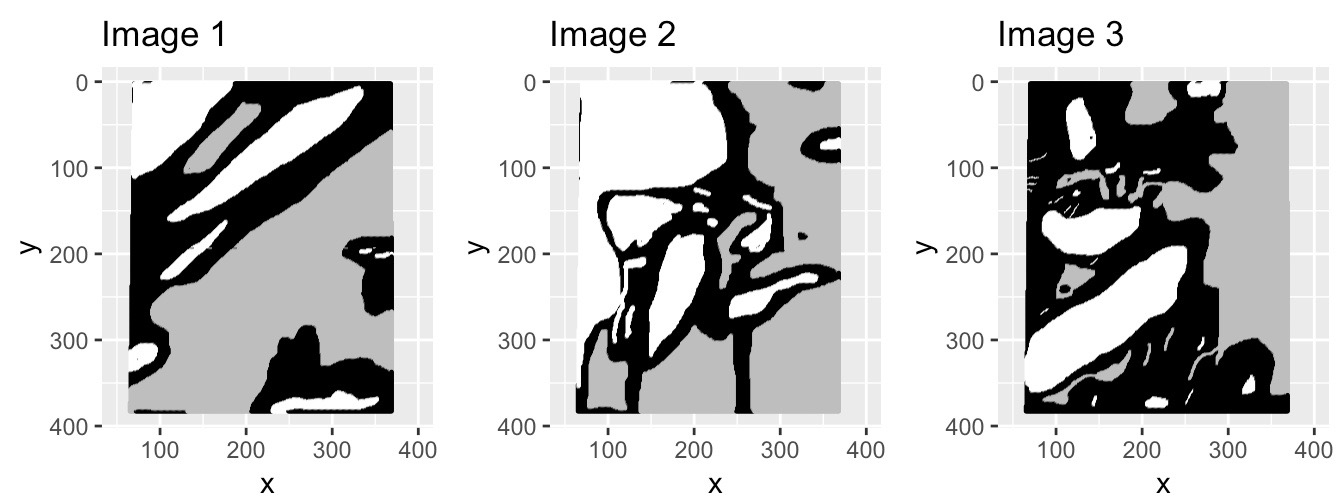
\includegraphics[scale=0.15,]{graphs-1}\caption{image photograph}\end{figure} 

\subsection{c) Exploratory data analysis}
For EDA, we use \textbf{correlation plot}, \textbf{principle component analysis}, and \textbf{histogram} to explore the data.\\
\indent First, we use \textbf{correlation plot} to present comprehensively the correlation between columns of features. We can observe that NDAI is positively correlated with SD and expert label (not very strong correlation though), but negatively correlated with all the rest features. DF,AF,AN,CF,BF are positively correlated with each other, which is very intuitive because they are radiance angles for the same image so they should be correlated. Their correlation also validates that the camera is functioning normally. We also notice that y coordinate is more related to radiance reading than x coordinate.
\begin{figure}[H]\hspace*{-1cm} \centering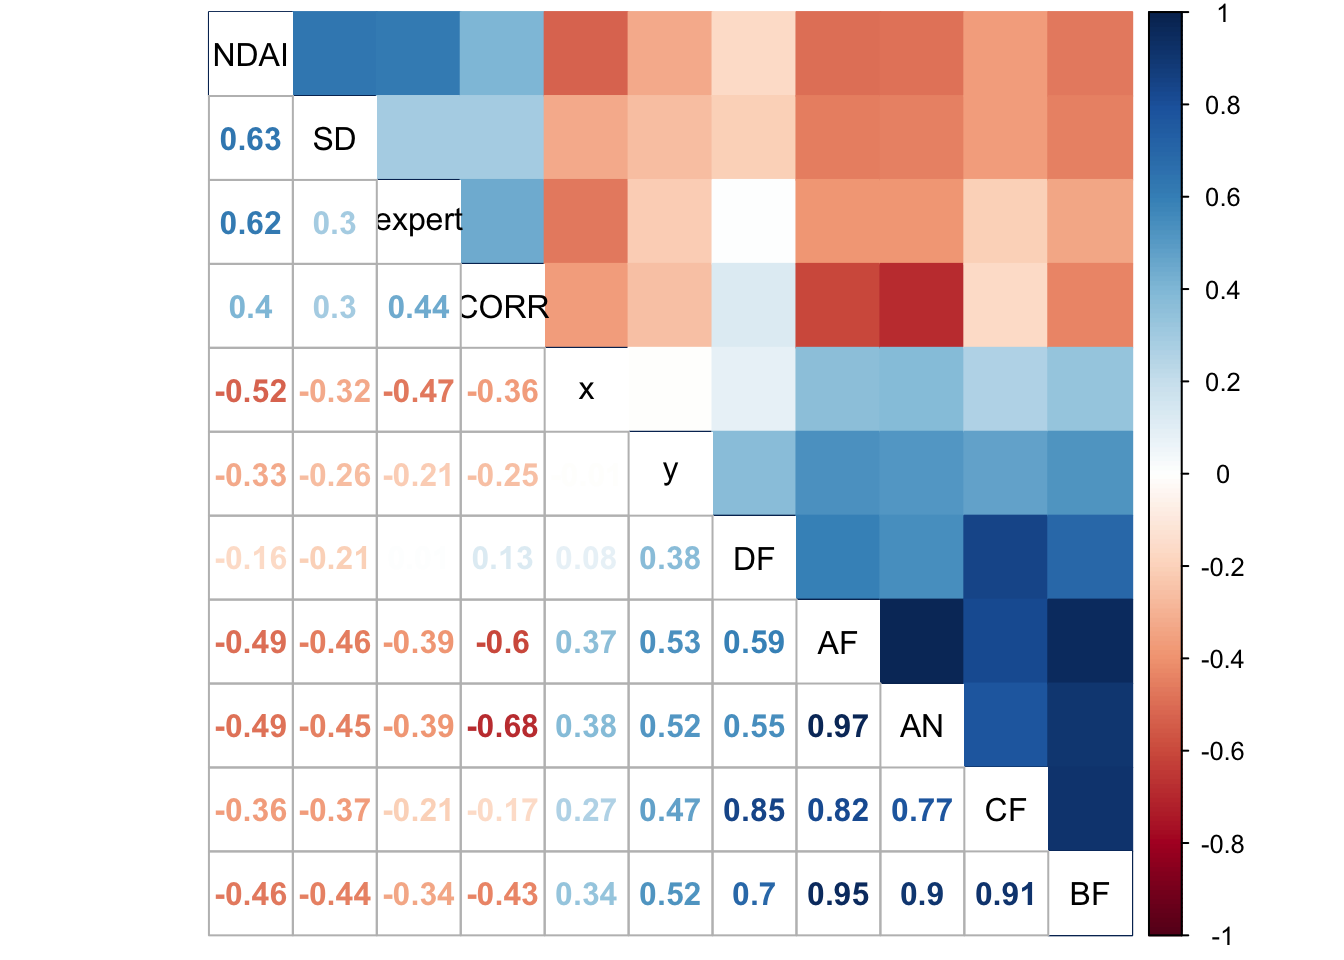
\includegraphics[scale=0.15,]{overallcorrelogram-1}\caption{correlogram}\end{figure}
\indent Second, we use \textbf{PCA} to examine the what dimensions contribute the most to the variance of the data. For simplicity, we only choose five features of the data, the five radiance angles. Quantitatively, we have five principle components whose summary is provided below, where \% of var shows the amount of variance each components alone explains and cum \% of variance shows the amount of variance all previous components explain:
\begin{verbatim}
  eigenvalue          % of var 		    cum % of variance
comp 1 4.22826569     84.5653137           84.56531
comp 2 0.61008098     12.2016195           96.76693
comp 3 0.10495903     2.0991807            98.86611
comp 4 0.04168339     0.8336678            99.69978
comp 5 0.01501091     0.3002183            100.00000
\end{verbatim}
We can see clearly that the first two component explains the majority of the variance. The first principal component captures 84.6\% of variance. first two principal component together capture above 96\% of the variability. To see it visually, we present the scree plot:
\vspace*{-0.1cm}\begin{figure}[H]\hspace*{-1cm} \centering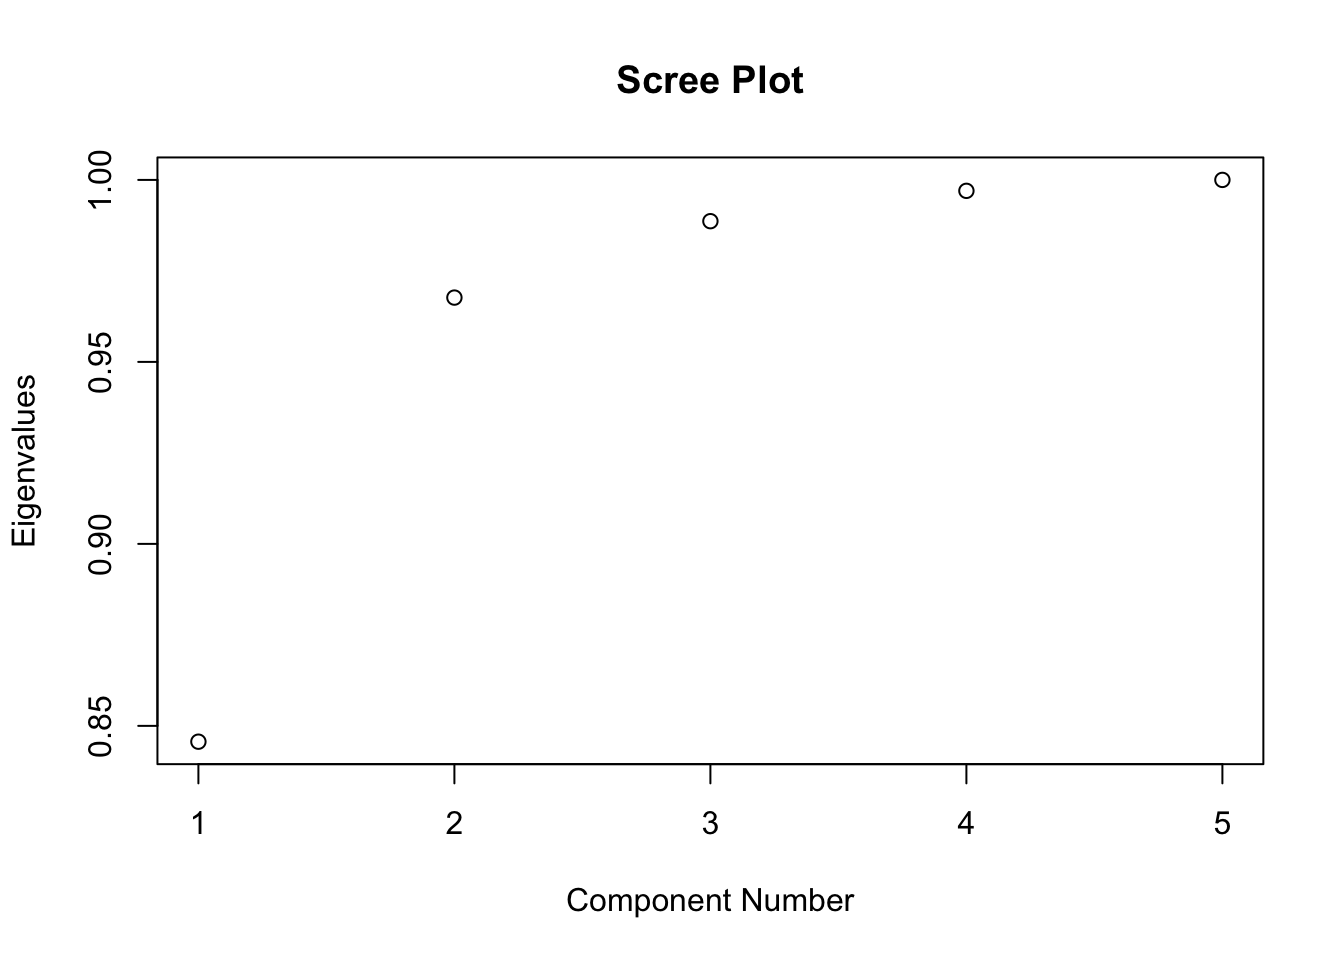
\includegraphics[scale=0.15,]{PCAamongradiance-2}\caption{scree plot}\end{figure}
Taking the first two principle component, we can examine how much each feature contribute to them. We now focus on the five radiance angles and plot them as vectors on the space spanned by the first two PCs.
\vspace*{-0.1cm}\begin{figure}[H]\hspace*{-1cm} \centering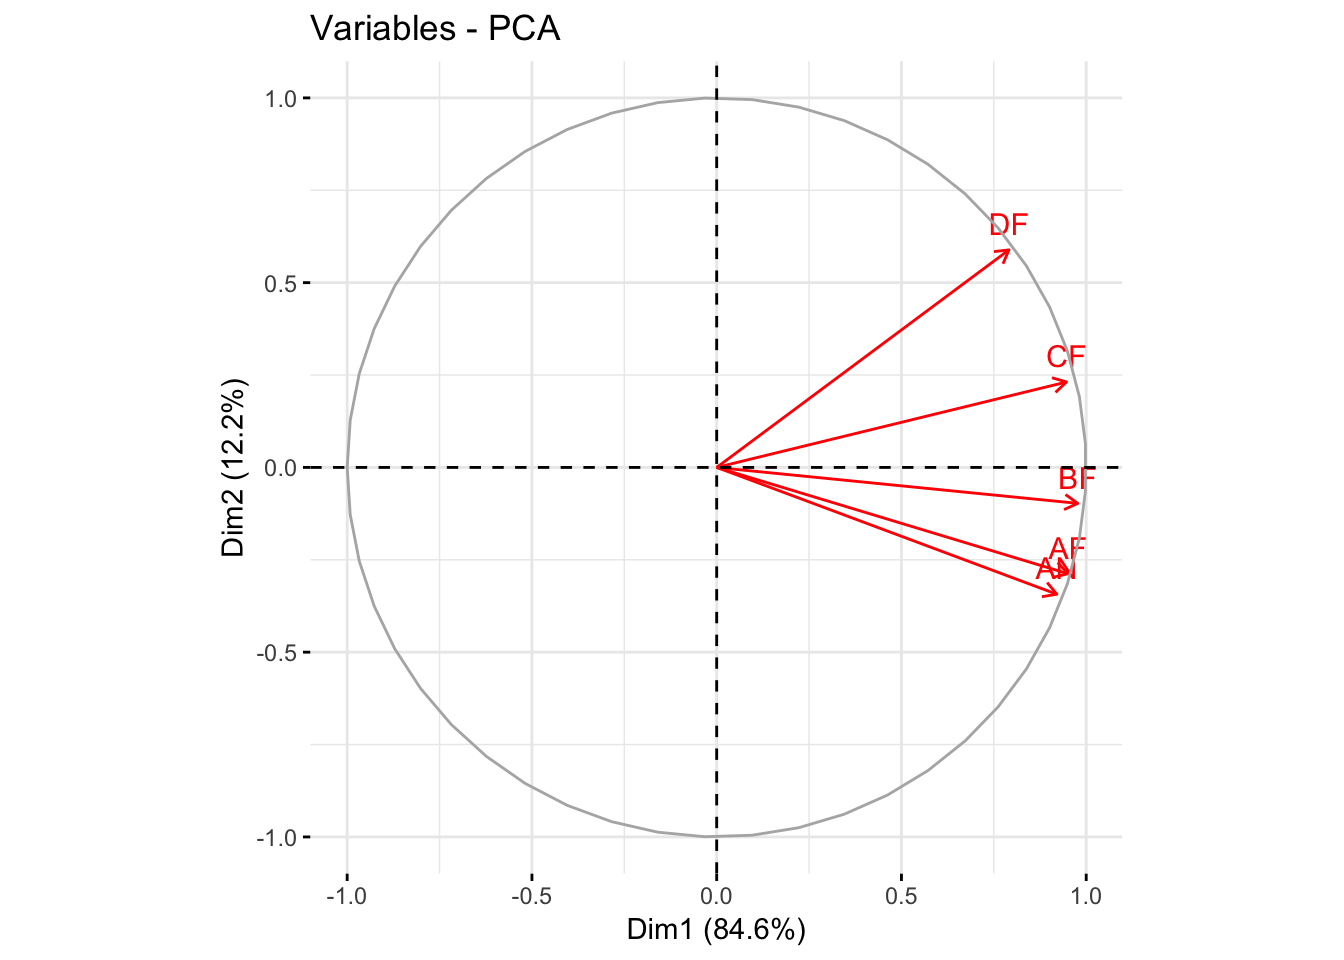
\includegraphics[scale=0.15,]{PCAamongradiance-1}\caption{Radiance Variance}\end{figure}

Each vector in the plot has a projection to the y axis and to the x axis. The projection to the x axis represents the correlation between PC1 and this feature, and the projection to the y axis represents correlation between PC2 and this feature. Because all five vectors point to the right, we can see that they correlate to PC1 to a very similar extent. The upshot is, because these five radiance angles correlate with the primary PC (PC1) so similarly, they alone do not offer additional explanation to the variance of the data apart from the other four radiance angle. This indicates that studying the radiance readings themselves may not have much results. NDAI, SD, and CORR comes to salvage the lack of explanatory power of the radiance angle.\\
\indent Now, we present some \textbf{histograms} of the data which further demonstrate that the NDAI feature created by Yu Bin and her team is very brilliant in terms of capturing the changes in a scene with changes in the MISR view direction.
\begin{figure}[H]
\hspace*{-.5cm}\begin{subfigure}{0.4\columnwidth}
    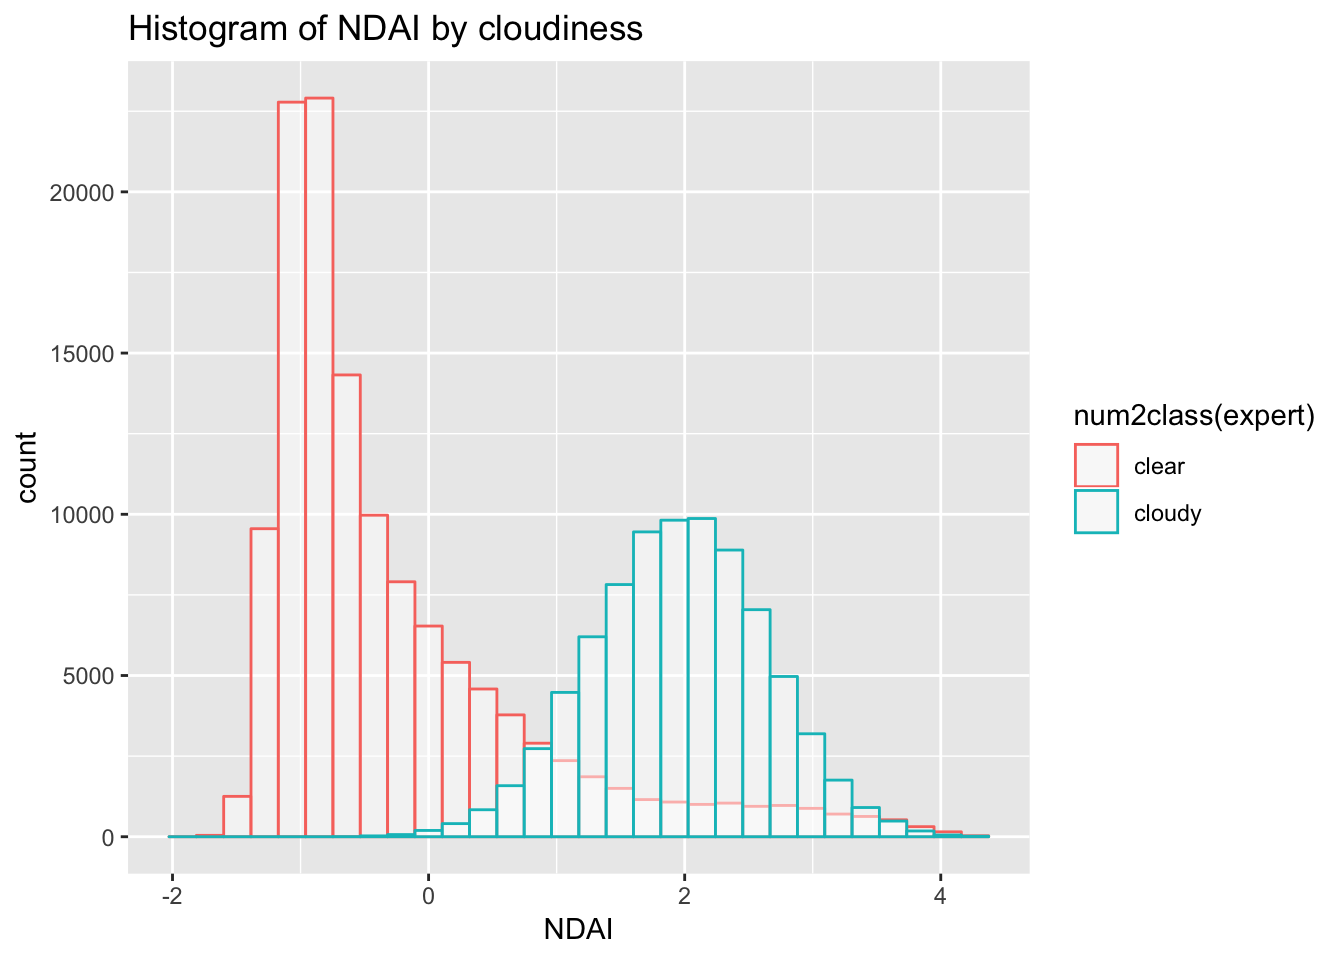
\includegraphics[scale=.1]{NDAI}
    \caption{NDAI}
    \label{fig:1}
  \end{subfigure}\hfill
\begin{subfigure}{0.4\columnwidth} \hspace*{-1cm}
    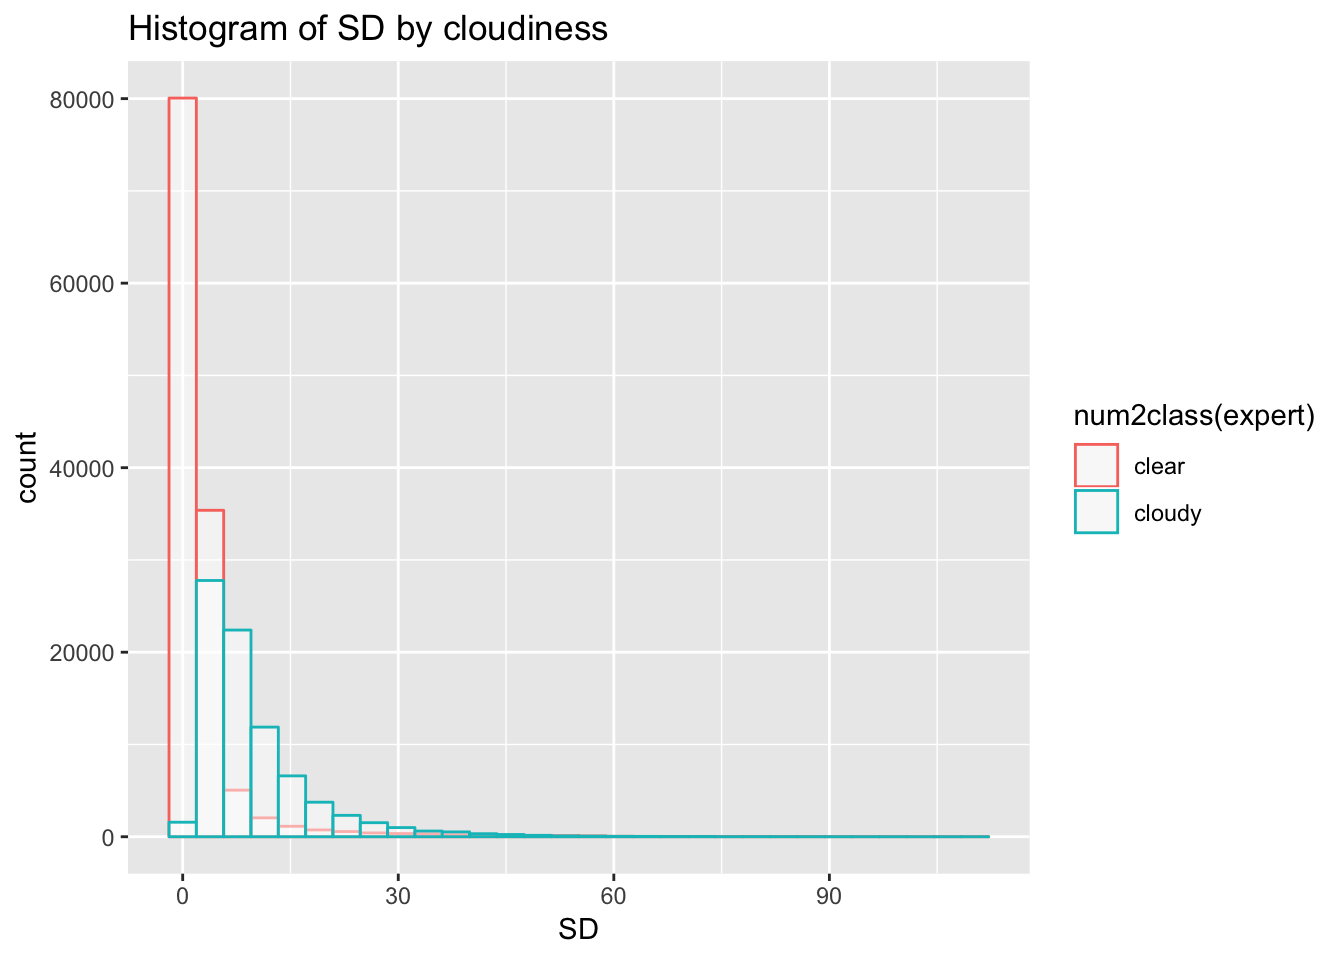
\includegraphics[scale=.1]{SD}
    \caption{SD}
    \label{fig:2}
  \end{subfigure}
  \begin{subfigure}{0.4\columnwidth} \hspace*{-0.5cm}
    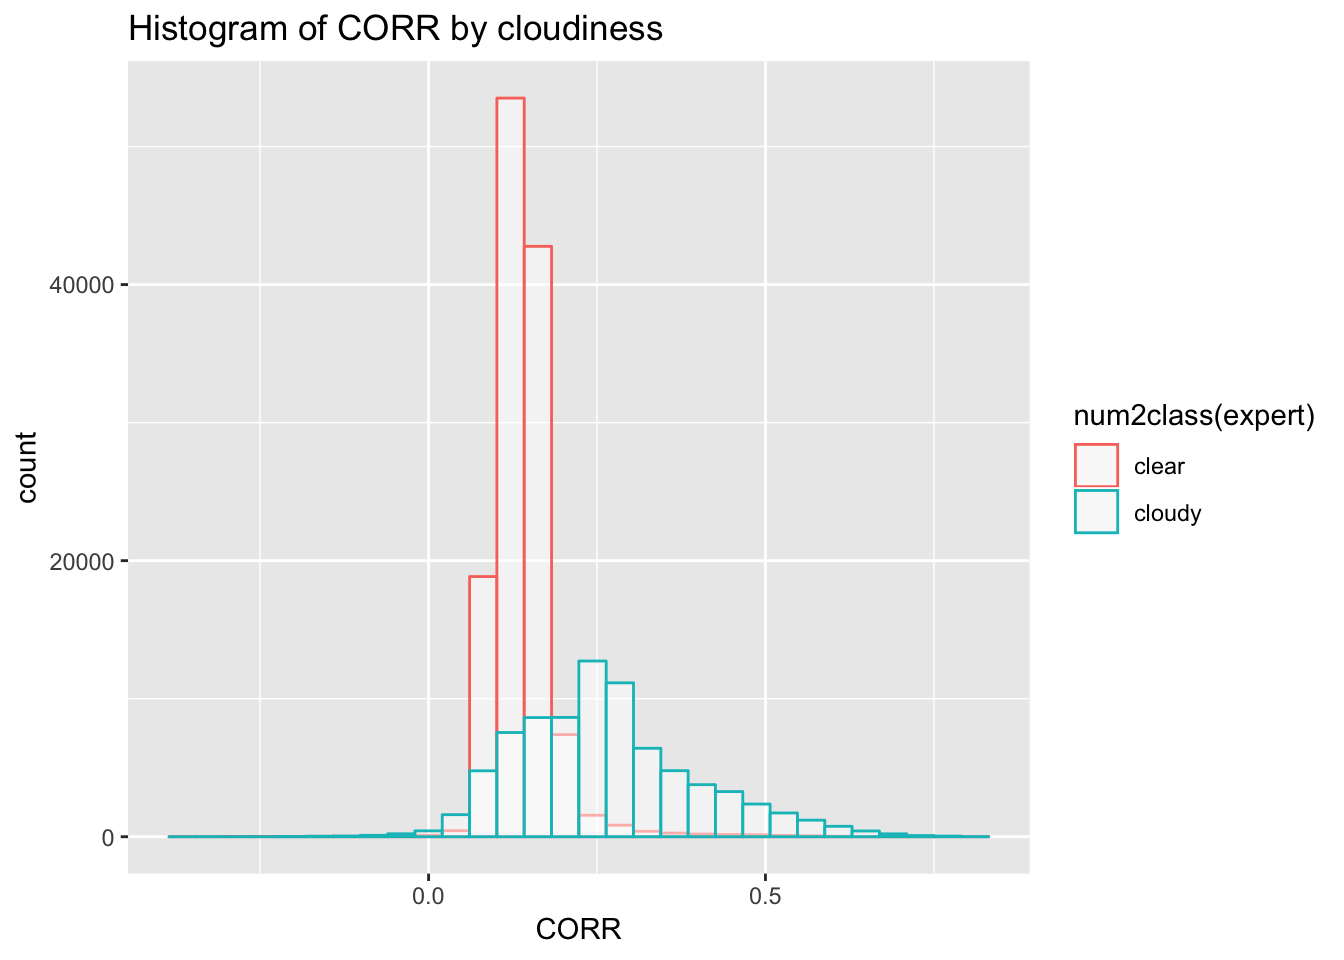
\includegraphics[scale=.1]{CORR}
    \caption{CORR}
    \label{fig:2}
  \end{subfigure}
 \caption{features}
\end{figure}


As shown above, most of the pixels in cloudy regions have high NDAI (the green histogram) and most of the pixels in clear regions have low NDAI (the red histogram). Here is a quantitative summary for the histogram where the first row is about the cloudy region and the second row is about the clear region:
\begin{verbatim}
  Min. 1st Qu.  Median    Mean 3rd Qu.    Max. 
-0.5855  1.4936  1.9613  1.9496  2.4120  4.3460 
   Min. 1st Qu.  Median    Mean 3rd Qu.    Max. 
-1.8420 -0.9756 -0.6555 -0.2627  0.1081  4.3387 
\end{verbatim}

The histogram for SD, as shown above in figure 5b), also forms a relatively well separation between two classes. Most cloudy regions have higher SD. However, the distribution is positively skewed and has long tail, which shows that the entire distribution is very squeezed in the lower end of SD. Comparatively, the cloudy region has a longer tail and a smaller peak. Here is a quantitative summary for the histogram where the first row is about the cloudy region and the second row is about the clear region:
\begin{verbatim}
   Min. 1st Qu. Median  Mean   3rd Qu. Max. 
 0.3825 4.5864  7.3006  9.8448 12.1102 99.2677 
   Min. 1st Qu. Median  Mean   3rd Qu. Max. 
 0.1987 0.8608  1.4351  2.9785 2.6157  110.4676 
\end{verbatim}
The histogram for CORR is shown above in figure 5c). Most cloudy regions have high CORR and their distribution is more spread out whereas the distribution of the clear region is more concentrated. However, the distribution of the clear region has a much lower peak than the distribution of the cloudy region. Here is a quantitative summary for the histogram where the first row is about the cloudy region and the second row is about the clear region:
\begin{verbatim}
   Min. 1st Qu.  Median    Mean 3rd Qu.    Max. 
-0.3537  0.1677  0.2531  0.2630  0.3331  0.8144 
   Min. 1st Qu.  Median    Mean 3rd Qu.    Max. 
-0.3617  0.1155  0.1359  0.1401  0.1617  0.7207 
\end{verbatim}
\vspace*{-0.1cm}\begin{figure}[H]\hspace*{-0.5cm} \centering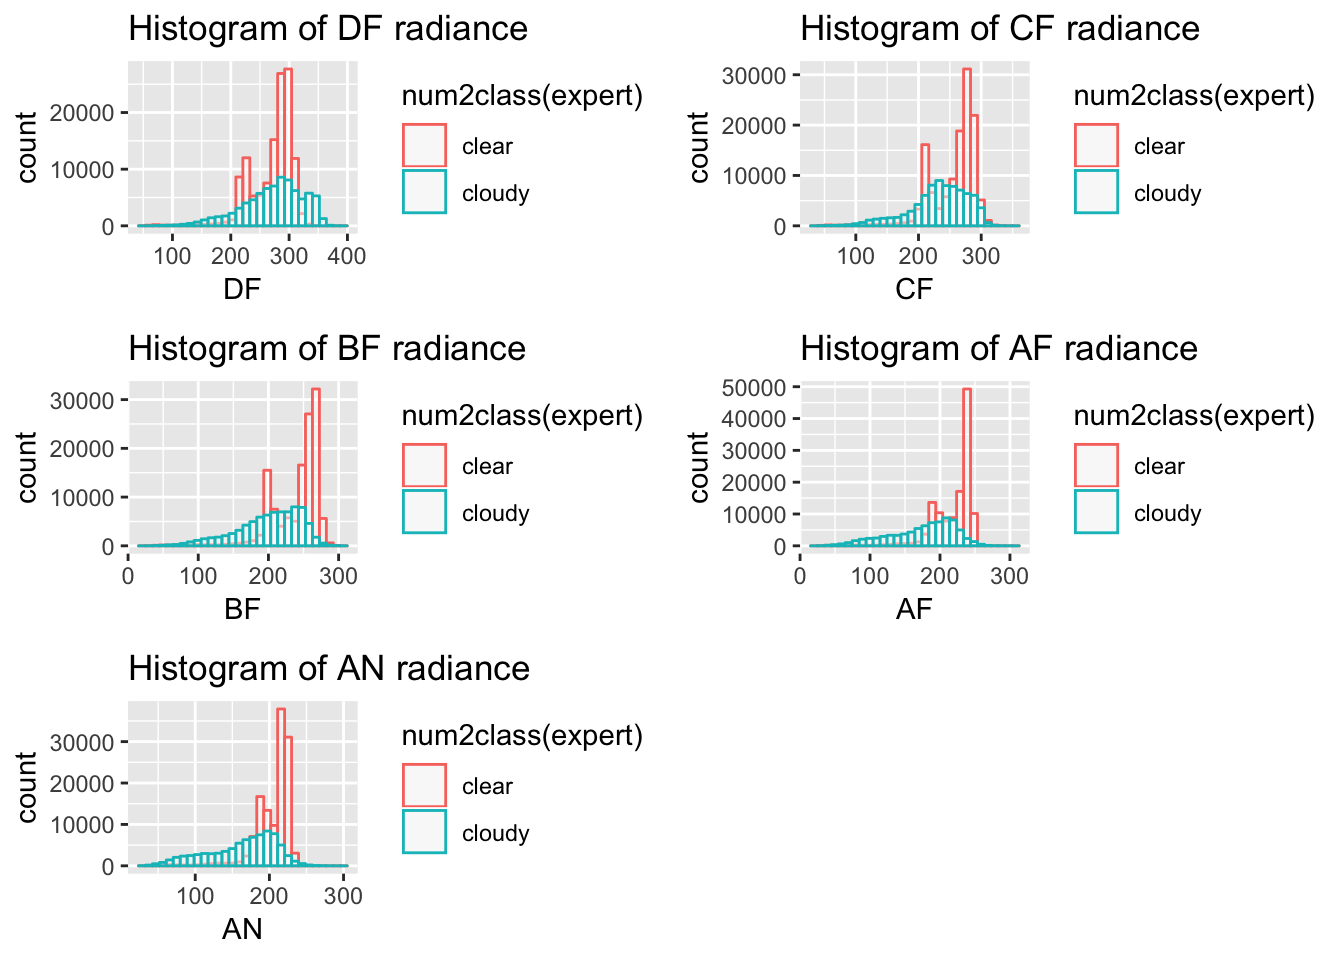
\includegraphics[scale=0.17,]{radiance}\caption{Radiance Angles}\end{figure}
As observed in the histogram of radiance angles presented above, they are the worst feature in classifying the two regions. The green histogram and the red histogram do not differ much and the histogram of all the radiance angles are very similar. 
clear areas seem to have a bimodal histogram of all of the radiance reading because there are two peaks, while cloudy areas have single-mode histogram of radiance reading. Cloudy areas have longer left-side tails but the clear region has higher peaks which means that clear areas seem to have slightly higher radiance reading (this is consistent with the paper finding as well).\\
\indent Although it is unwise to use them to train classifiers, it resonates our analysis in PCA that they provide us with confident that the measurement camera functions normally so we can trust our dataset.

\section{\textbf{Part II: Preparation}}
\subsection{a) Data Split}
We have three ways of splitting the data: \textbf{divide and forge}, \textbf{divide and sample}, and \textbf{image blurring}. As observed in the previous part, the data is not iid because the pixels close to the cloudy pixels tend to be cloudy. These methods all take into consideration of this fact and reduce the level of dependency between pixels.\\
\indent \textbf{divide and forge} and \textbf{divide and sample} start by carving each image into subimages. We decided to choose 36 as the number of subimages for each image. It is implemented by equally dividing the horizontal edge and the vertical edge of the image by six parts. In combination, they yield $6 \times 6$ subimages. In total, we have $3 \times 36 = 108$ subimages because we have 3 images. Now, the two methods differ in that \textbf{divide and forge} forms the training set by stratified random sampling whereas \textbf{divide and sample} forms the training set by simple random sampling. The form the training data, the former assumes it to be a image, just like image 1, 2, or 3. To construct this image, we sample for each subimage that constitutes it. For example, to obtain the subimage of the top-left corner, we sample from $\{image1, image2, image3\}$. If we get, say, image 1, we use the corresponding top-left subimage from image 1 to fill in this blank. We perform the same procedure for all the 36 subimage of the training set. Together, they constitute our training set image. Similarly, we can use the same procedure for the validation and testing set. The \textbf{divide and sample} does not assume the training set to be a image. It simply randomly sample 36 subimages out of the total 108 subimages to be the training set and similarly randomly sample for the validation and testing set. Because the subimages may come from the same corner of the original image, there is no guarantee we can reforge them into images. Both methods reduce the dependency by aggregating pixels into subimages. Even though the pixels are dependent on their neighbors, the subimages are much less dependent on other subimages. For example, it is probable that one subimage may have 56\% clouds but the next only 3\%.\\
 \vspace*{-0.1cm}\begin{figure}[H]\hspace*{-0.5cm}\centering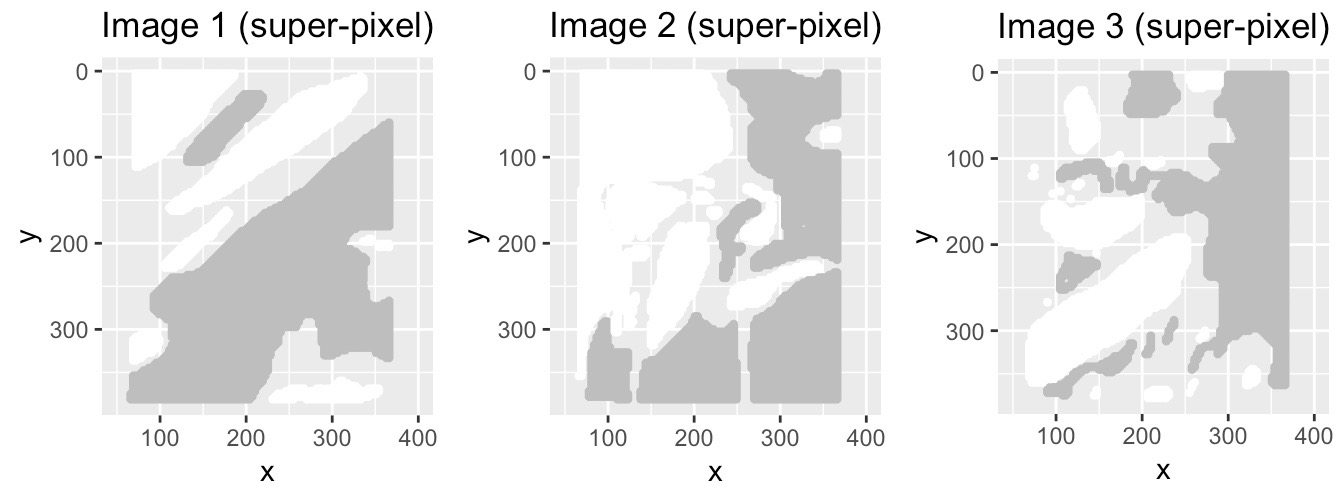
\includegraphics[width = 8cm, height = 3cm]{blur}\caption{Blurred images}\end{figure}
\indent The third method, which is later proven to be the best one, is \textbf{image blurring}. It groups all the pixels in an image by 9 and average them into a superpixel. So the features of each superpixel is obtained by averaging 9 original pixels. It's as if we blurred the original image. To form training, validation, and testing set, we simply randomly sample from the superpixels. Each superpixels are less dependent on others because the features of each pixel is averaged by the ones of the pixels most dependent on it, namely its 8 neighbors. In forming superpixels, we already consider the most dependent cluster of pixels as one pixel and thus it is less dependent upon other cluster of pixels. The downside of this method is by blurring, we reduce the data size. But later on we'll see it is not a problem. Here are the blurred images consisting super pixels which resemble the original images.



\subsection{b) Accuracy of the Trivial Classifier}
The best splitting method's accuracy using a trivial classifier (a classifier that classifies everything as clear region) should be around the true percent of "clear" label in the entire given data, because it indicates that our split is not biased towards clear region nor cloudy region. The trivial classifier will have high accuracy if the data split is not good in the sense that it splits almost all the terrain into the testing data. It is the only occasion where the trivial classifier obtains high accuracy. However, this splitting is problematic because it does not represent the reality. Our first method of splitting the data (\textbf{divide and forge}) yields accuracy close to chance:
\begin{verbatim}
     val_accuracy test_accuracy
1         0.47324       0.73446
2         0.56654       0.60891
3         0.55805       0.66128
4         0.63969       0.58523
5          0.5908       0.66446
6         0.66373       0.66214
7         0.58254       0.66957
8         0.63268       0.53584
9          0.5896       0.68739
10        0.67056       0.54833
----    ---------     ---------
mean      0.59674       0.63576
sd        0.05871       0.06379
\end{verbatim}
Recall from part I that the percentage of clear amongst the labeled regions is about 61.08\%, which is close to the accuracy above (0.64). Therefore the trivial classifier is doing no better than chance, indicating it's also a non-trivial way to split the data. Because the trivial classifier does not do well according to our way of splitting the data, we can be more certain that our splitting method is not trivial and does a good job in representing the whole data.\\
\indent Noticeably, this method has different average accuracy on validation and testing, indicating that validation set is slightly different from the testing set (in terms of \% clear labels). This is probably associated with the "stratified sampling" idea we incorporated. However, since the difference is within 1 sd; it's also very likely due to chance. Therefore, we do not think this is an evidence against such method. We then observe that divide and forge's sd significantly decreased, after we increase K from 4 to 6 (K is the number of divides along each axis). Such low sd (high stability) makes method 2 very appealing. But it could also mean that such method is very dependent on how many sections we divide.
\indent Similarly, the trivial classifier fails in our second method \textbf{divide and sample}: 
\begin{verbatim}
     val_accuracy test_accuracy
1         0.66324       0.54433
2         0.52452       0.58367
3         0.59933       0.58026
4         0.67523       0.65689
5         0.54647       0.69146
6         0.55698       0.52426
7         0.68942       0.56331
8         0.69759       0.59633
9         0.54607       0.70142
10        0.68164       0.68775
----    ---------     ---------
mean      0.61805       0.61297
sd        0.06985       0.06562
\end{verbatim}
This method has higher sd than the previous one because it is simple random sampling. However, it has average accuracy very similar across validation and testing. But the accuracy is still close to chance so this method is also non-trivial.
\indent Our third method \textbf{image blurring} also passes this test:
\begin{verbatim}
     val_accuracy test_accuracy
1         0.60541       0.61105
2         0.61053       0.61197
3         0.61355       0.60541
4         0.61053       0.60331
5         0.60659        0.6062
6         0.60554       0.60383
7         0.60685       0.60515
8         0.60711       0.61433
9         0.60908       0.61407
10        0.60987        0.6041
----    ---------     ---------
mean      0.60851       0.60794
sd        0.00264        0.0044
\end{verbatim}
Splitting method three is the most stable one according to the trivial classifier because the sd is very low and the validation accuracy is very close to test accuracy, while other methods have quite different accuracy across validation and testing. Apparently, the accuracy is not better than chance so \textbf{image blurring} is also a valid splitting method. We will be using \textbf{image blurring} as the splitting method for the following parts.


\subsection{c) First Order Importance}
We choose two criteria as the preliminary criteria for feature important: \textbf{separation between class mean}, and \textbf{correlation with expert label}. To obtain both criterion, we first standardize the data without centering the mean. The first criterion is obtained by first separating each feature data into two classes according to the expert label, then calculating the mean in each class, and lastly subtract the two means. Intuitively, the larger the difference, the more separated the means are and the more separated the means are, the better the feature is at classification. Because if the data of a feature centers at very distinct values for two classes, it is more readily to tell, according to this feature, that which class does a data point belongs to. Just see how close it is to one of the means. If two means are too close, a data point could be very close to both means and we can hardly tell which class it belongs to. The second criterion is obtained by calculating the correlation between each feature and the expert label. Apparently, the higher the correlation, the better the feature is a predicting the class to which a data point belongs. If it is better at predicting the class label, it is usually a better feature to train a classifier with.\\
\indent We know in advance that the position cannot contribute to explaining where is cloudy and where is not. Clouds may move anywhere. It is simply a contingent fact. For the first criterion (10a) and the second criterion (10b), we can plot a histogram for all the feature but x and y:
\begin{figure}[H]
\hspace*{-.5cm}\begin{subfigure}{0.4\columnwidth}
    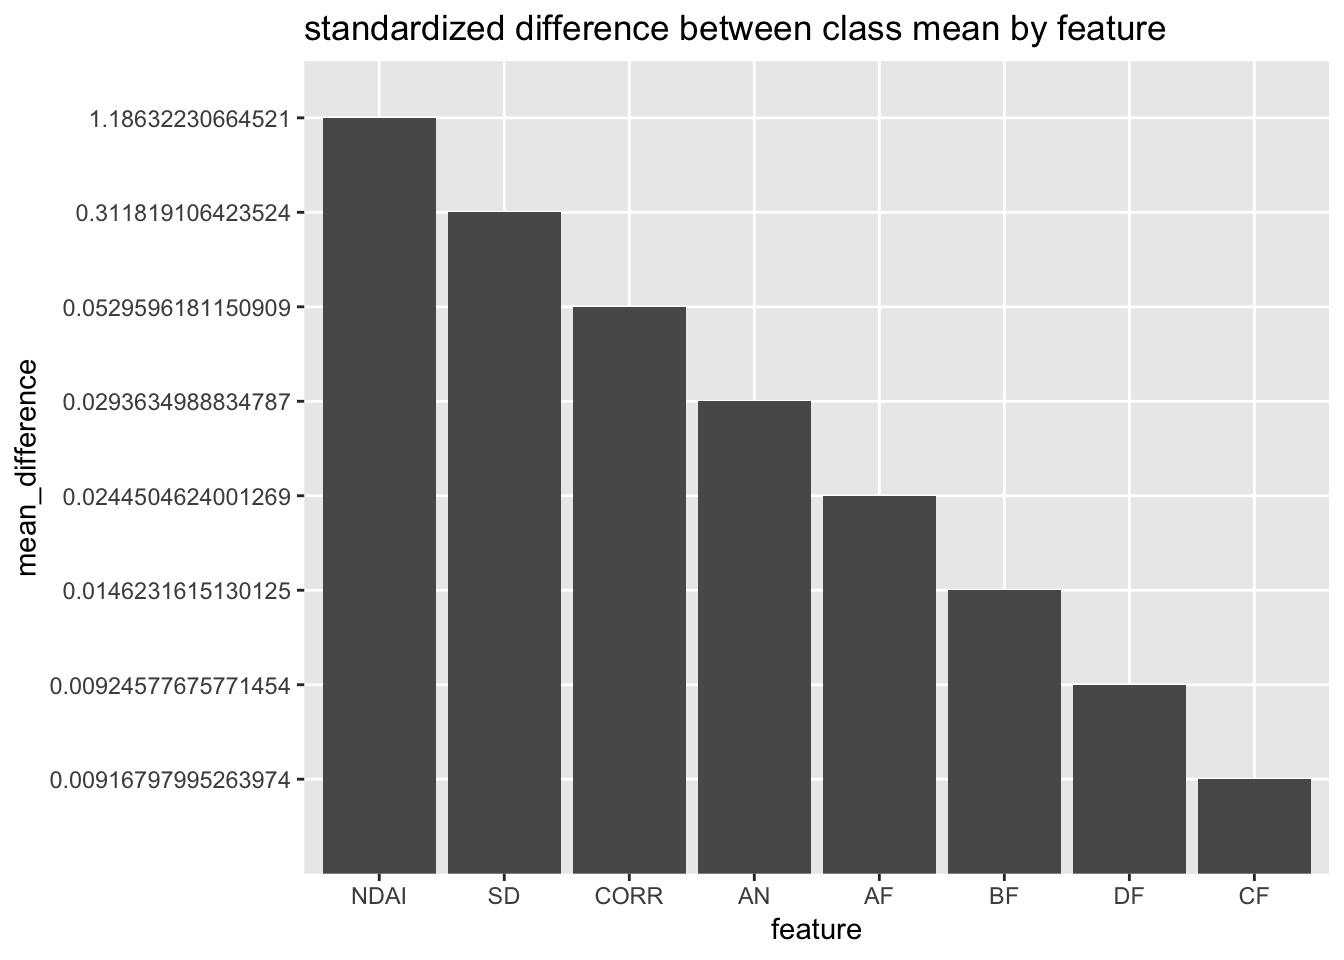
\includegraphics[scale=.1]{mean}
    \caption{separation of mean}
    \label{fig:1}
  \end{subfigure}\hfill %%
\begin{subfigure}{0.4\columnwidth} \hspace*{-1cm}
    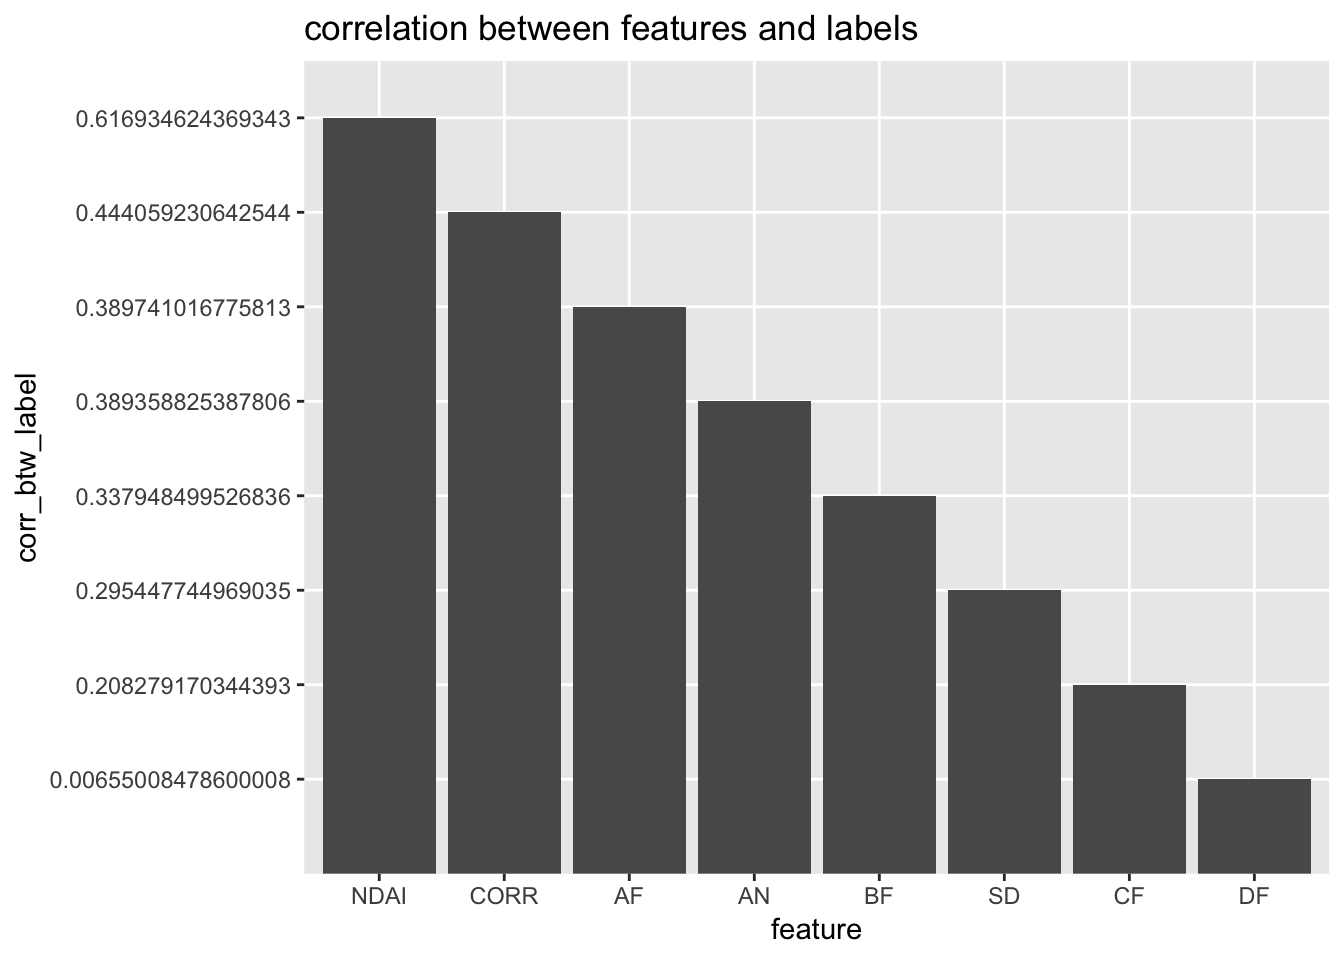
\includegraphics[scale=.1]{correlation}
    \caption{correlation}
    \label{fig:2}
  \end{subfigure}
 \caption{two criteria}
\end{figure}

Then quantitatively for 10a), we have:
\begin{verbatim}
  feature     mean_difference
1    NDAI    1.18632230664521
2      SD   0.311819106423524
3    CORR  0.0529596181150909
4      DF 0.00924577675771454
5      CF 0.00916797995263974
6      BF  0.0146231615130125
7      AF  0.0244504624001269
8      AN  0.0293634988834787
\end{verbatim}
Obviously in 10a) NDAI, SD, and CORR rank the highest and thus they are the best three features according to this criterion. The second criterion yields similar outcome:
quantitatively for 10b), we have:
\begin{verbatim}
  feature      corr_btw_label
1    NDAI   0.616934624369343
2      SD   0.295447744969035
3    CORR   0.444059230642544
4      DF 0.00655008478600008
5      CF   0.208279170344393
6      BF   0.337948499526836
7      AF   0.389741016775813
8      AN   0.389358825387806
\end{verbatim}
The trend is very similar between the two criteria. In both criteria, NDAI and CORR rank on the top. However, in the second criterion, SD scores a bit lower which indicates that even though two classes are very far way according to SD (the second farthest), SD is not extremely correlated with the expert labels. Overall NDAI and CORR are the main feature for classification and SD can be the extra feature that offers help in increasing separability.

\subsection{d) CV Generic Function}
For detail, check out our code in Github.

\section{\textbf{Part III: Modeling}}
\subsection{a) Classification Methods with Cross Validation}
We choose four classification methods: \textbf{Linear Discriminant Analysis}, \textbf{Quadratic Discriminant Analysis}, \textbf{Logistic Regression}, and \textbf{Decision Trees}. We first explain the assumptions behind each method.\\
\indent \textbf{Linear Discriminant Analysis (LDA)} assumes that the data points are generated independently and identically from a mixture Gaussian distribution with the same variance. In our case, the mixture Gaussian is composed by two Gaussian distributions with the same covariance matrix but different means. One corresponds to the cloudy region and the other corresponds to the clear region. Each data point has a probability that it's generated from the cloudy Gaussian and a probability that it's generated from the clear Gaussian. Therefore, each data point has a pair of posterior probabilities corresponding to the Gaussian distribution of each class. LDA regards class corresponding to the higher posterior as the class that the data point belongs to. The boundary between two classes is a linear plain due to the assumption that two Gaussian variances are the same. \textbf{Linear Discriminant Analysis (QDA)} also assumes that the data is generated by a mixture Gaussian, but the variance of the two Gaussian is not assumed to be the same. Therefore the boundary is not linear but quadratic. We cannot tell whether the assumptions of LDA and QDA are met, because there is no way to find out the "true" mechanism of data generation in nature. We can only see if these two methods give us a good fit to the data. However, we do not think that the independence assumption is not met. But with our innovative way of splitting the data, we can assume that they are independent.\\
\indent For \textbf{Logistic Regression}, many assumptions are cut. However, it still requires the data to be independent and it also functions by assuming a binomial distribution. Additionally, independent variables should not be too highly correlated with each other if we want to use logistic regression. The independence problem is dealt by data splitting and overall, NDAI, SD, and CORR are not correlated except NDAI and SD. The correlation between NDAI and SD is 0.63, which is relatively high. So this assumption is not well met. \textbf{Decision Trees} assumes very few things. Because it is a non-parametric method, it assume no background distribution. More importantly, it does not assume independence between data. In short, this method does not assume anything that is crucial to the application of the method.\\
\indent Now, I present the result of fitting each classification method to the data cross validated by two splitting method we presented earlier (the question only asks for two). For \textbf{image blurring}, we have:
\begin{verbatim}
            LDA     QDA     GLM    Tree
1       0.90092 0.90617 0.90748 0.91142
2        0.9101 0.91732 0.88903 0.90157
3       0.91732 0.90026 0.88969 0.91798
4       0.89823 0.92186 0.90354 0.90945
5       0.90617 0.89823 0.90157 0.90814
6       0.89888  0.8956 0.89961 0.90217
7       0.90414 0.89567 0.90289 0.89494
8       0.91339 0.90945 0.90414 0.90879
9       0.90414 0.90748 0.90617 0.92257
10      0.91601 0.90348 0.89494 0.91787
------- ------- ------- ------- -------
average 0.90693 0.90555 0.89991 0.90949
\end{verbatim}
All methods have a relatively high accuracy in predicting the testing data. Decision tree has the highest accuracy, and then LDA, and then QDA, and GLM (logistic regression) ranks the lowest. However, the difference between their performance is slim. Also the accuracy in different folds are not much different, so there is no one particular fold that is outrageous. \\
For another splitting method \textbf{divide and forge}, we have:
\begin{verbatim}
            LDA     QDA     GLM    Tree
1       0.89886 0.89733 0.89134 0.90569
2       0.89635 0.90339 0.89196 0.90297
3       0.89496 0.89928  0.8921 0.90471
4       0.89593 0.90373 0.89384 0.90199
5       0.89621 0.89823 0.89377 0.90116
6        0.8951 0.89969 0.89126 0.90443
7         0.899 0.90095 0.89092 0.90359
8       0.89608 0.89879 0.89496 0.90756
9       0.89329 0.90004 0.89273 0.90729
10      0.89621 0.90109 0.89036  0.9029
------- ------- ------- ------- -------
average  0.8962 0.90025 0.89232 0.90423
\end{verbatim}
All methods have a relatively high accuracy in predicting the testing data still. Decision tree remains to have the highest accuracy, and then QDA, and then LDA, and GLM (logistic regression) ranks the lowest. However, the difference between their performance is still slim. Also the accuracy in different folds are not much different, so there is no one particular fold that is outrageous.\\

\subsection{b) Model Comparison with ROC}
The ROC curve plots the true positive (y-axis) against the false positive (x-axis). In another word, the y-axis represents the percentage of the data that belong to this class and actually get classified into the class. The x-axis is the percentage of the data that does not belong to this class and still get classified into the class. In general, we want to maximize the true positive, i.e., to have as many data actually in the class to be classified in, and minimize the false positive, i.e., to have as few data not in the class to be classified in. The point that best satisfies this requirement is (0, 1). However, in reality, (0, 1) is almost never on the actual ROC curve. Then we face a trade-off: how devastating are false positives. If we can tolerate many false positive, but we want the true positive to be as high as possible, we can choose the points that are further to the right on the ROC curve. On the other hand, if even one false positive can be devastative, we may want to choose points that are leaning towards the left on the ROC curve. In our problem, we are uncertain which axis we care more so we consider them equally important. Mathematically, we want the point on the ROC that is closest to (0, 1). Whatever model parameter corresponding to this point gives us the best parameter according to ROC curve. Here is the ROC plot for all the classification methods:\\ 
\begin{figure}[H]\hspace*{-0.5cm} \centering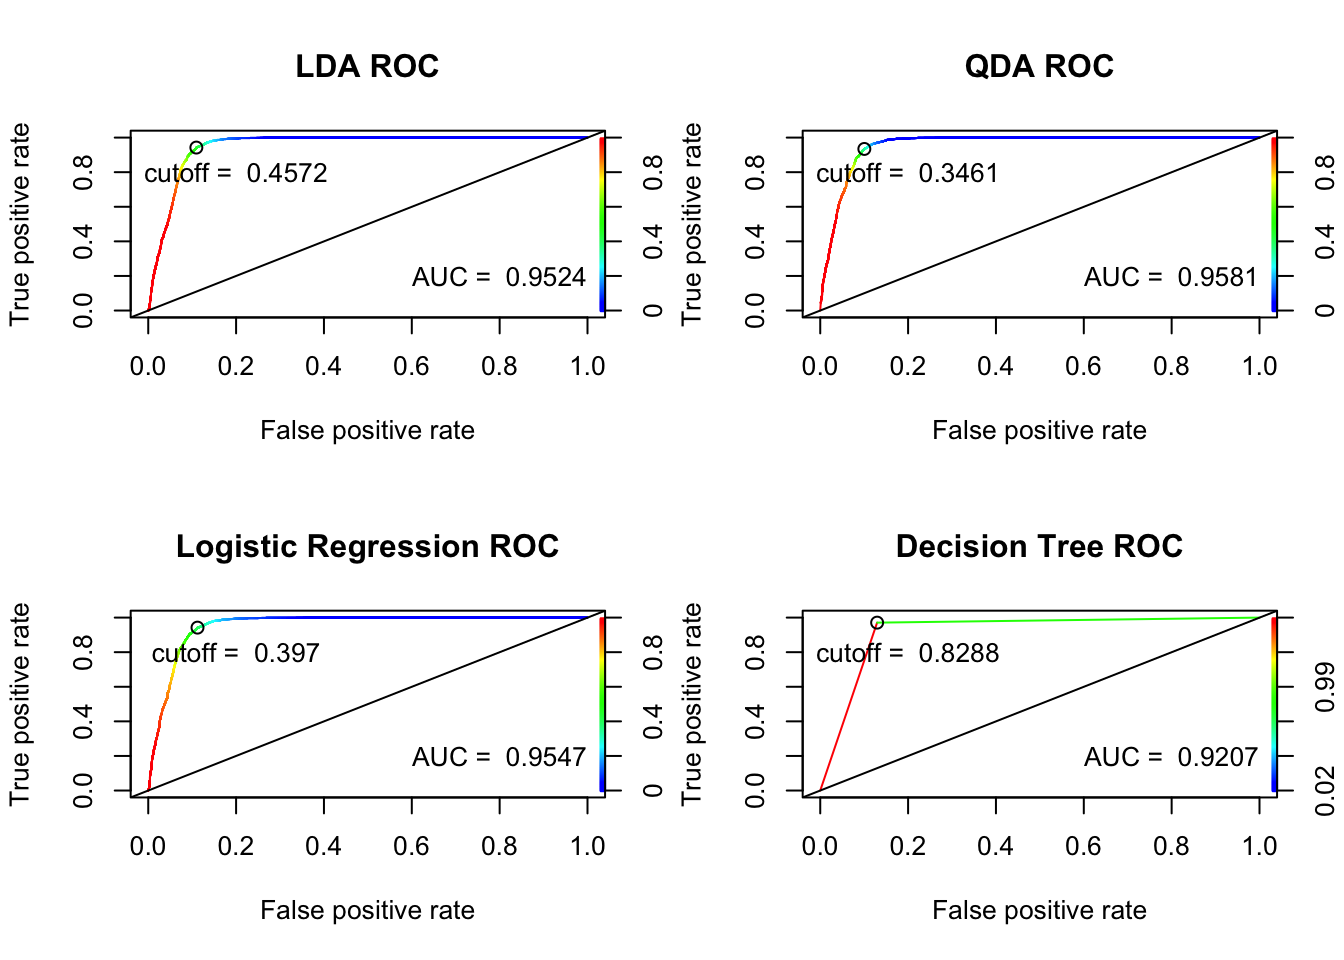
\includegraphics[scale=0.2,]{ROC}\caption{ROC plot}\end{figure}
\indent We want to choose the cutoff that corresponds to point closest to the ideal point (0, 1) where we classify correctly everything truly in the class and we do not classify in anything that is not in the class. According to the curve, the best cutoff for LDA is 0.4572, for QDA is 0.3461, for Logistic Regression is 0.397, and for Decision Tree is 0.8288.\\
\indent The ROC curve also provides insight to model comparison. We want to choose the model that maximizes the AUC, which is the area under the ROC curve. It is maximized by QDA whose ROC is 0.9581. The area is a good criterion for model comparison because the larger the area, the closer the curve is to the top line $y = 1$ and the y-axis $x = 0$. Ideally, the curve is composed of only these two lines which means for any cutoff, we always have perfect true positive. However, in reality it is always a trade-off because the lower the false positive is, the lower the true positive as well. Therefore a model is better if each under low false positive, the true positive is still high, which is translated into attaining the maximal AUC. 


\subsection{c) Model Comparison with AIC, BIC (bonus)}
Alternatively, we can also compare these methods with AIC and BIC. Because AIC and BIC only apply to methods assuming a background distribution generating the sample data, we cannot use it on decision tree which does not assume background probability distribution. Both AIC and BIC are calculated as the log likelihood (llh) that our sample data is generated by the probability assumed by the model while penalizing for model complexity measured by number of parameters. It is a way to compare with model assumes a more plausible probability distribution. Intuitively, the one assuming a better probability distribution which generates the sample data with high llh is the better one. Let k be the number of parameter, n be the sample size, the formula for AIC and BIC is: 
$$AIC = -2llh + k$$ $$BIC = -2llh + log(n)k$$
The AIC and BIC can be easily calculated for the logistic regression because r has built-in information. We spent spent days and nights trying to find built-in AIC, BIC, llh, or the variance of the fitted mixture Gaussian for LDA and QDA. Finally, we decide to calculate and estimate every quantity by hand. To do so, we use the fact that LDA and QDA both assume the data is generated by a mixture Gaussian distribution. Hence the likelihood of each data point is a weighted average of the Gaussian corresponding to the class of cloudy region and the Gaussian corresponding to the class of clear region, weighted by the prior. Most of the necessary parameters are obtained from r but we estimated the covariance matrix by hand. To get the llh of each data point, we simply take the log of the likelihood. To get the llh of the entire data set, we can simply add up the llh for each data point because our splitting method has already dealt with the dependency of the data. The only difference between LDA and QDA is that for LDA, there are only 6 parameters: the mean and prior of the first Gaussian, the mean and prior of the second, and the shared covariance matrix. For QDA, there are 7 parameters because the covariance matrix for both distribution is not assumed to be the same. Here are the AIC and BIC:
\begin{verbatim}
##               LDA   QDA logistics
## AIC_result 108162 84301    7859
## BIC_result 108205 84353    7890
\end{verbatim}
The result is stunning. LDA and QDA are much higher in AIC and BIC than the logistics regression and the higher a model in AIC and BIC, the worse fit the model is. Nevertheless, recall the AUC of the ROC graph, logistics regression is at least worse than QDA, but how can QDA be much worse than logistics regression according to LDA and QDA? One explanation is that the model assumption of QDA is very erroneous. The data is simply not generated by a Mixture Gaussian but somehow the classification is still accurate. Another possibility is that AIC and BIC are not a suitable metric for model comparison of classification methods. The model fit of the data is not essential for a task like classification. At least we tried this alternative metric and we learned from it.

\section{\textbf{Part IV: Diagnostics}}
\subsection{a) diagnosis of the QDA Method}
According to the model comparison in the part above, we decide to run diagnostics on the QDA method. We first plot the convergence plot of the training error of QDA against the training set size using our better splitting method, \textbf{image blurring}:
\begin{figure}[H]\hspace*{-2cm} \centering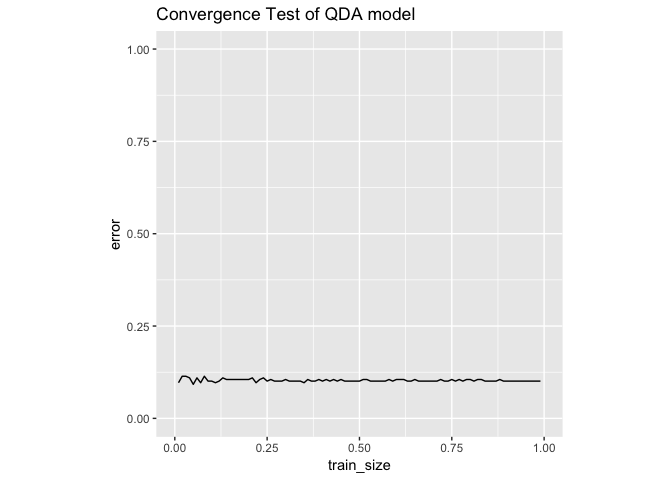
\includegraphics[width=12cm, height = 5cm]{convergeBlur}\caption{Error convergence according to blurring}\end{figure}
We see that QDA's error converge. According to the image blurring splitting, it has low error from the beginning and remain at that level (10\% error rate) regardless of the training sample size. Therefore QDA is fairly stable and the demand on training set size is not high.
\indent We can also take a look add the class mean and whether it converges as the training size increases: 
\hspace*{-1cm}\begin{figure}[H]\centering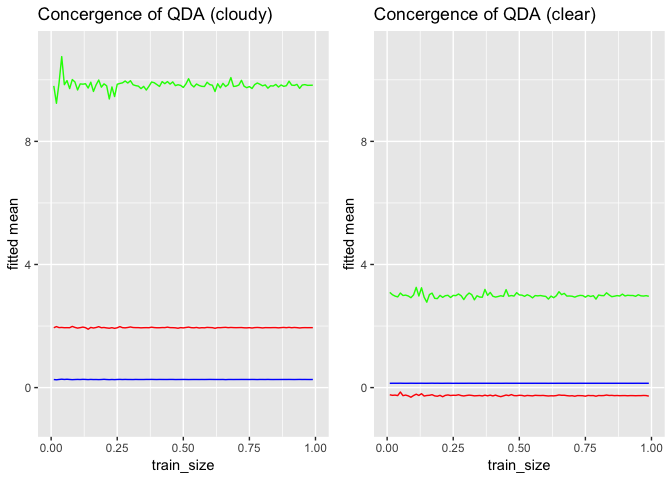
\includegraphics[width=8cm, height = 3cm]{convergeMean}\caption{Mean convergence}\end{figure}
The red line represents the class mean of NDAI, the blue line represents the class mean of CORR, and the green line represents the class mean of SD. We can see that all these mean in both classes converge really quickly as the training size increases. The mean of SD is more fluctuating but not for a hug extent.

Lastly, we can run diagnosis on the convergence of the cutoff value: 
\begin{figure}[H]\hspace*{-1.5cm}\centering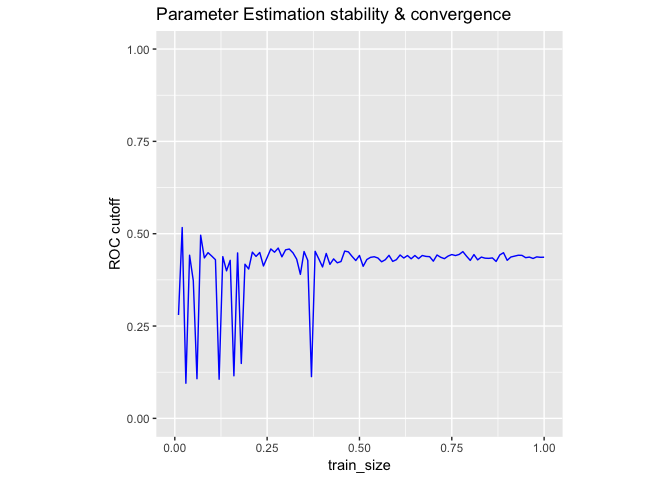
\includegraphics[width=12cm, height = 5cm]{convergeCutoff}\caption{Cutoff convergence}\end{figure}
As we can see, the best cutoff converges when the training size is about half of the entire data. Before that, the best cutoff is very unstable. Many dips keep occurring. Yet the cutoff eventually converges to about 40\%. 


\subsection{b) Pattern in Misclassification}
If we choose the image blurring as the splitting method, we do observe systematic misclassification, but the misclassification is not biases because the percentage of clear (cloudy) in the pool of misclassified is similar to the percentage of clear (cloudy) in the real data. Therefore we did not misclassify one class more than another:
\begin{verbatim}
##               clear    cloudy  
## misclassified "58.51%" "41.49%"
## total_labeled "61.08%" "38.92%"
\end{verbatim}
It is reasonable to suspect that systematic errors may come from abnormal feature values. Quantitatively, we indeed observe such anomaly:
\begin{verbatim}
##      false clear false cloudy
## NDAI  -1.4426236sd     2.499319sd
## SD    -0.5897147sd    1.905845sd
## CORR  -0.7801425sd     1.048086sd
\end{verbatim}
All three features are extremely skewed. The false clear (cloud misclassified as clear) has feature values almost 1 sd below that of the average cloud, and the false cloudy (clear misclassified as cloudy), in contrast has feature values almost 2 sd above that of the average clear. The NDAI is especially abnormal amongst all three feature. As shown before, NDAI is the most informative feature so such a abhorrent deviation in NDAI is especially devastating. But where exactly are these misclassified data located? Now, let us plot out the data that are misclassified and we see that there is a cluster which resembles a cloud in image 3: 
\begin{figure}[H]\centering\hspace*{-1cm}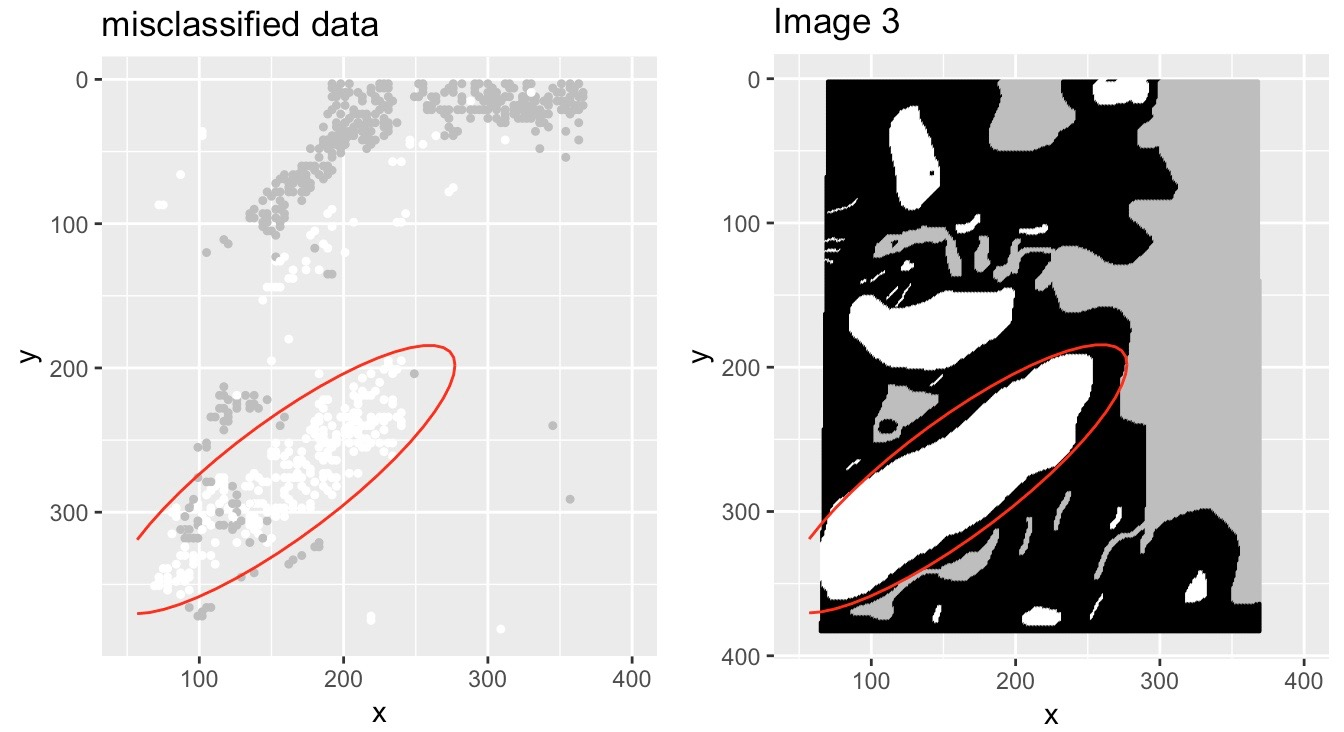
\includegraphics[width = 9cm, height = 4cm]{misclassify}\vspace*{-0.5cm}\caption{misclassified}\end{figure}

In the plot of misclassified data (trained with the original data based upon the image blurring method, not just with image 3), the white dots represent those that should be classified as cloud and yet misclassified as clear whereas the gray dots represent the vise versa. Apparently, most of the white dots form a shape (highlighted by the red oval) happen to be similar to this huge chunk of cloud in image 3, indicating that most of the cloud data misclassified as clear are from this cloud in image 3. This is perhaps because image 3 is taken at different place / different time, and image 3's cloud is somehow different from image 1 and 2. But most data comes from image 1 and 2, thus the model trained based on image 1 and 2 may not apply well to cloudy areas in image 3. For the clear parts that are misclassified, it's harder to find some evidence from this graph alone.\\
\indent To figure out why the systematic misclassification arises, we plot the histogram of all three features in the misclassified data. The distribution labeled "clear" means the data that are actually clear but falsely classified as cloudy, i.e. the false cloud, and The distribution labeled "cloud" means the data that are actually cloudy but falsely classified as clear, i.e. the false clear: 

% \begin{figure*}[H]
% \begin{subfigure}[b]{.4\textwidth}
% 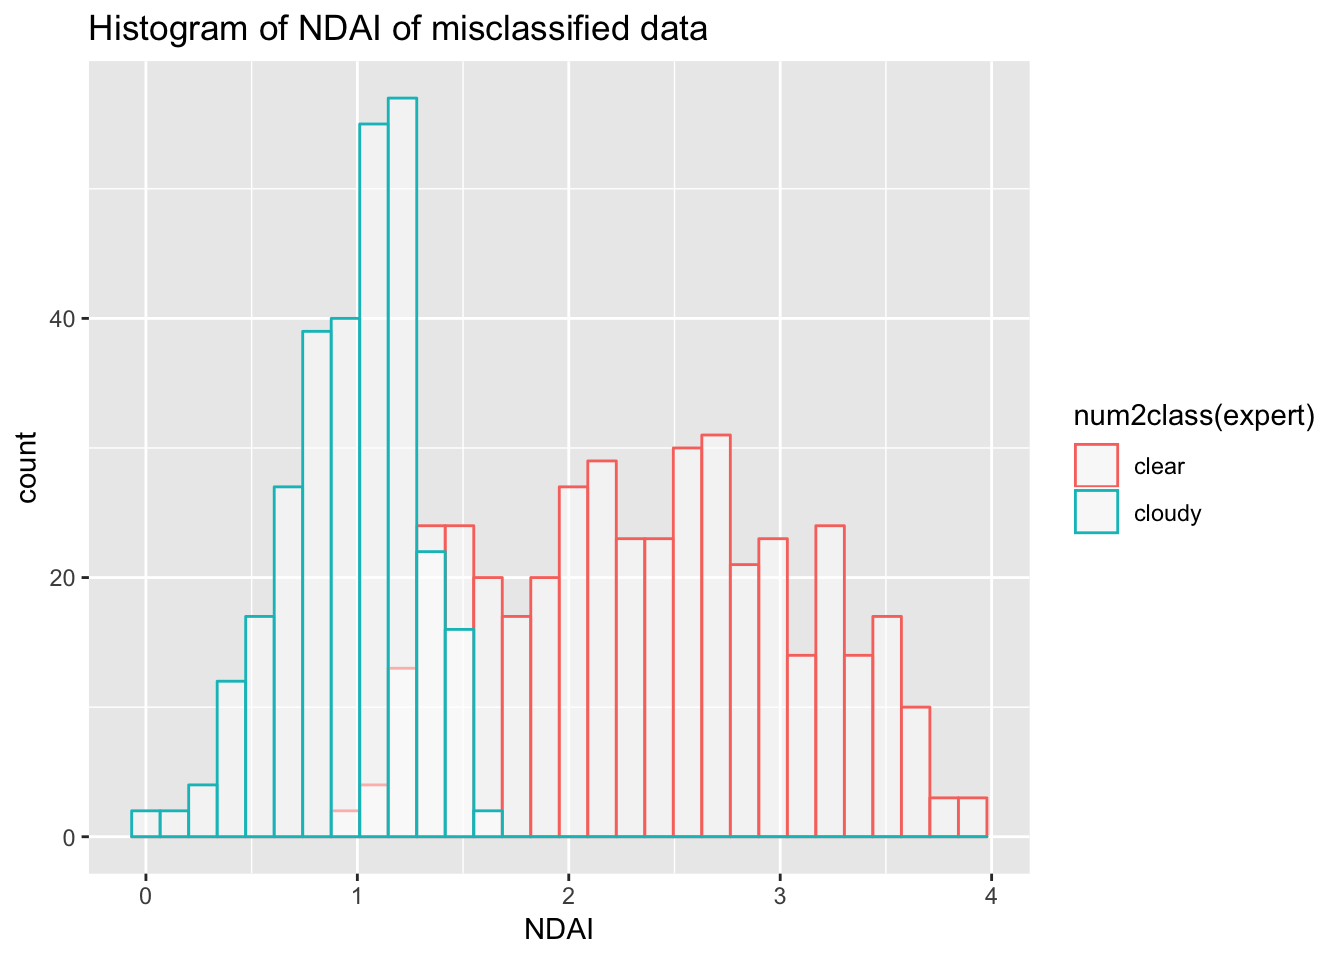
\includegraphics[scale=.1,]{NDAImis.png}
% % 	\caption{NDAI}
% \caption{Caption}\label{label-a}
% \end{subfigure}\qquad\qquad\qquad\qquad
% \begin{subfigure}[b]{.4\textwidth}
%  	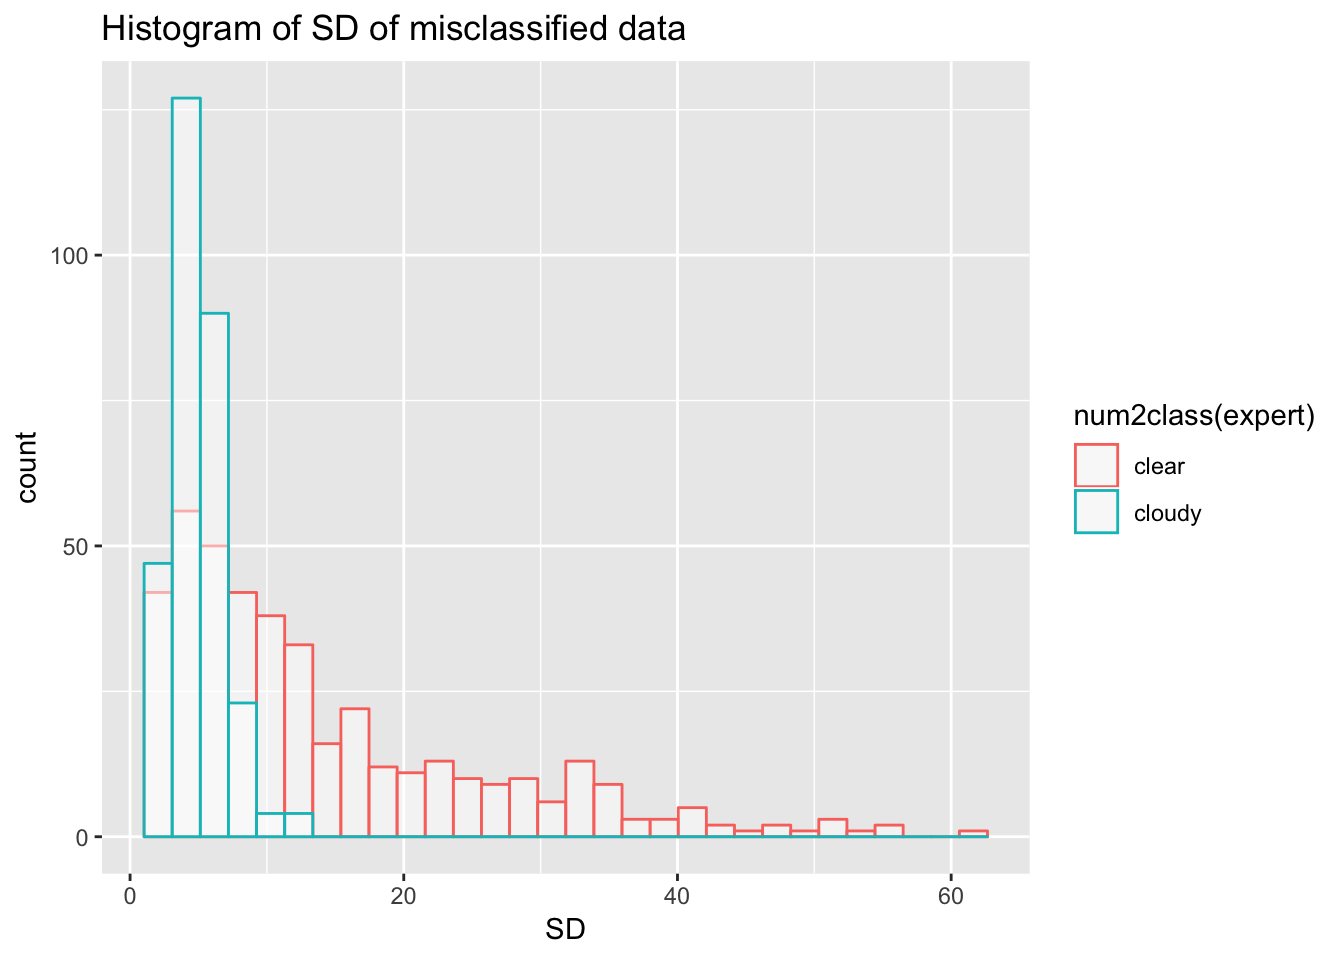
\includegraphics[scale=.1,]{SDmis.png}
% % 	\caption{SD}
% \caption{Caption}\label{label-b}
% \end{subfigure}
% \end{figure*}

\begin{figure}[H]
\hspace*{-.5cm}\begin{subfigure}{0.4\columnwidth}
    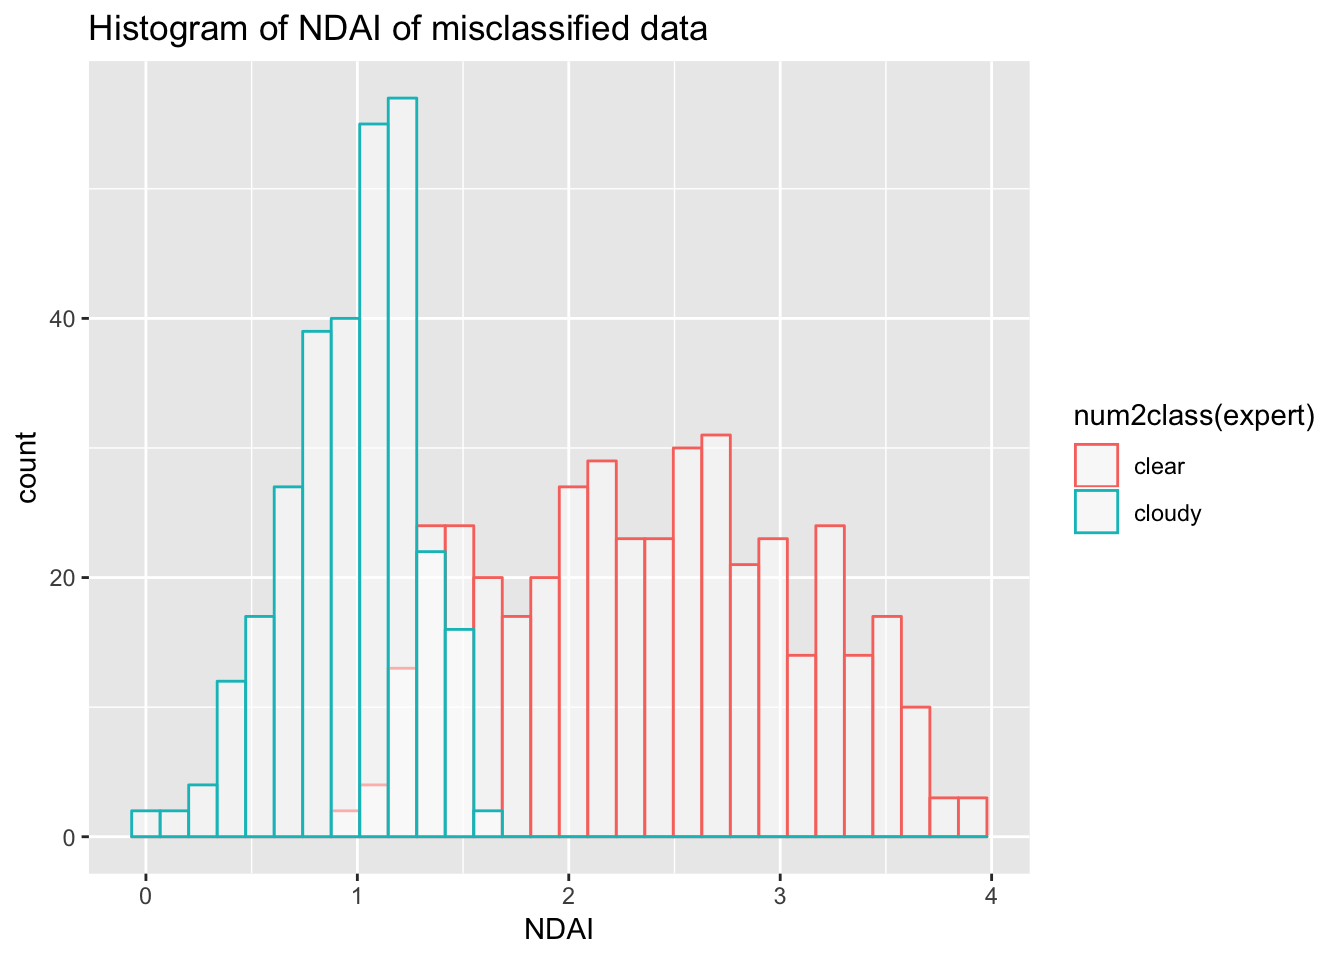
\includegraphics[scale=.1]{NDAImis}
    \caption{NDAI}
    \label{fig:1}
  \end{subfigure}\hfill %%
\begin{subfigure}{0.4\columnwidth} \hspace*{-1cm}
    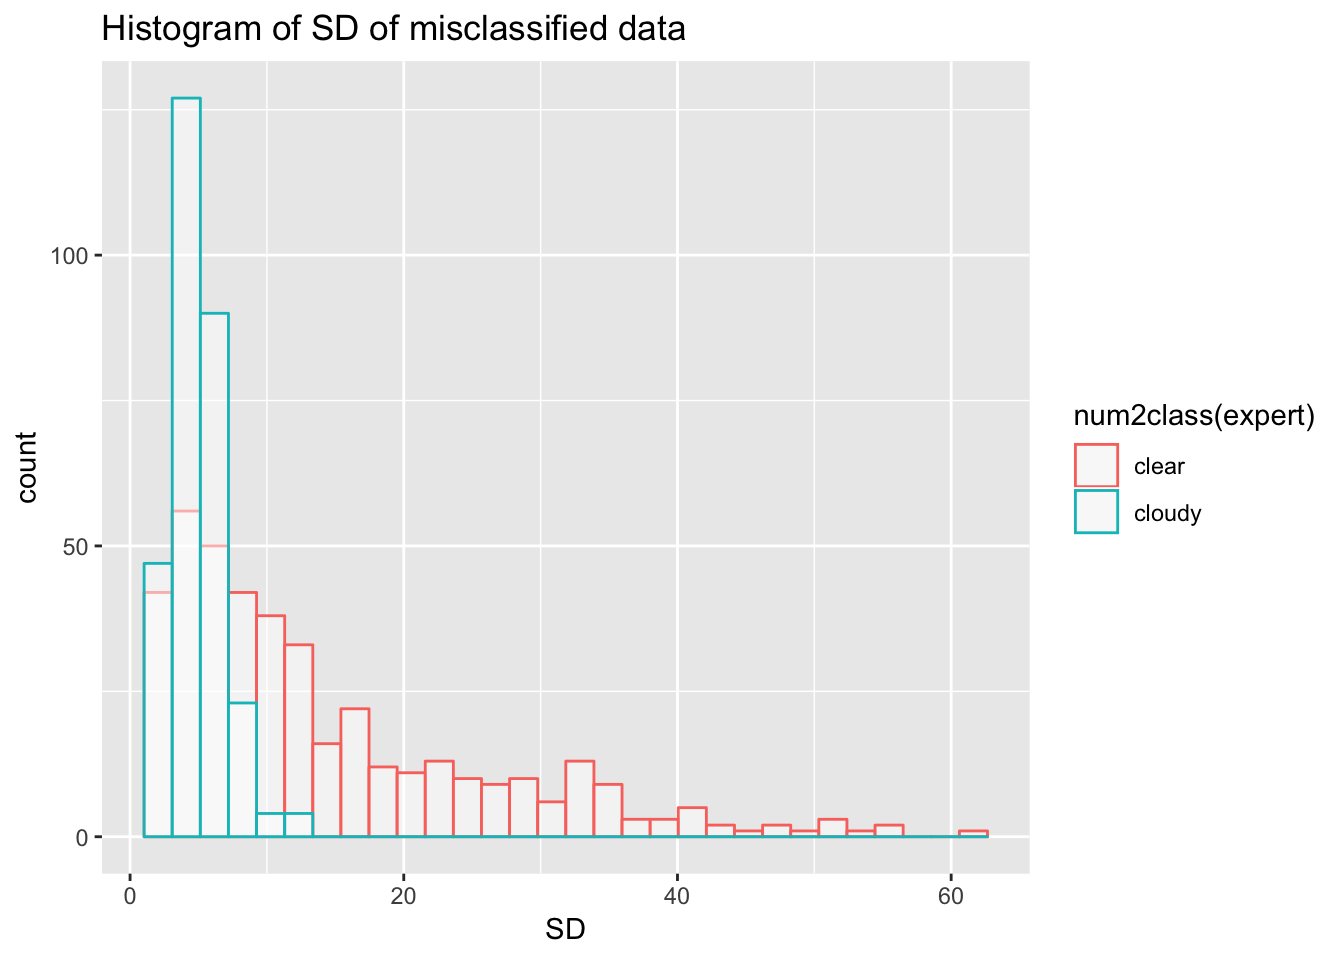
\includegraphics[scale=.1]{SDmis}
    \caption{SD}
    \label{fig:2}
  \end{subfigure}
\hspace*{-.5cm}\begin{subfigure}{0.4\columnwidth}
    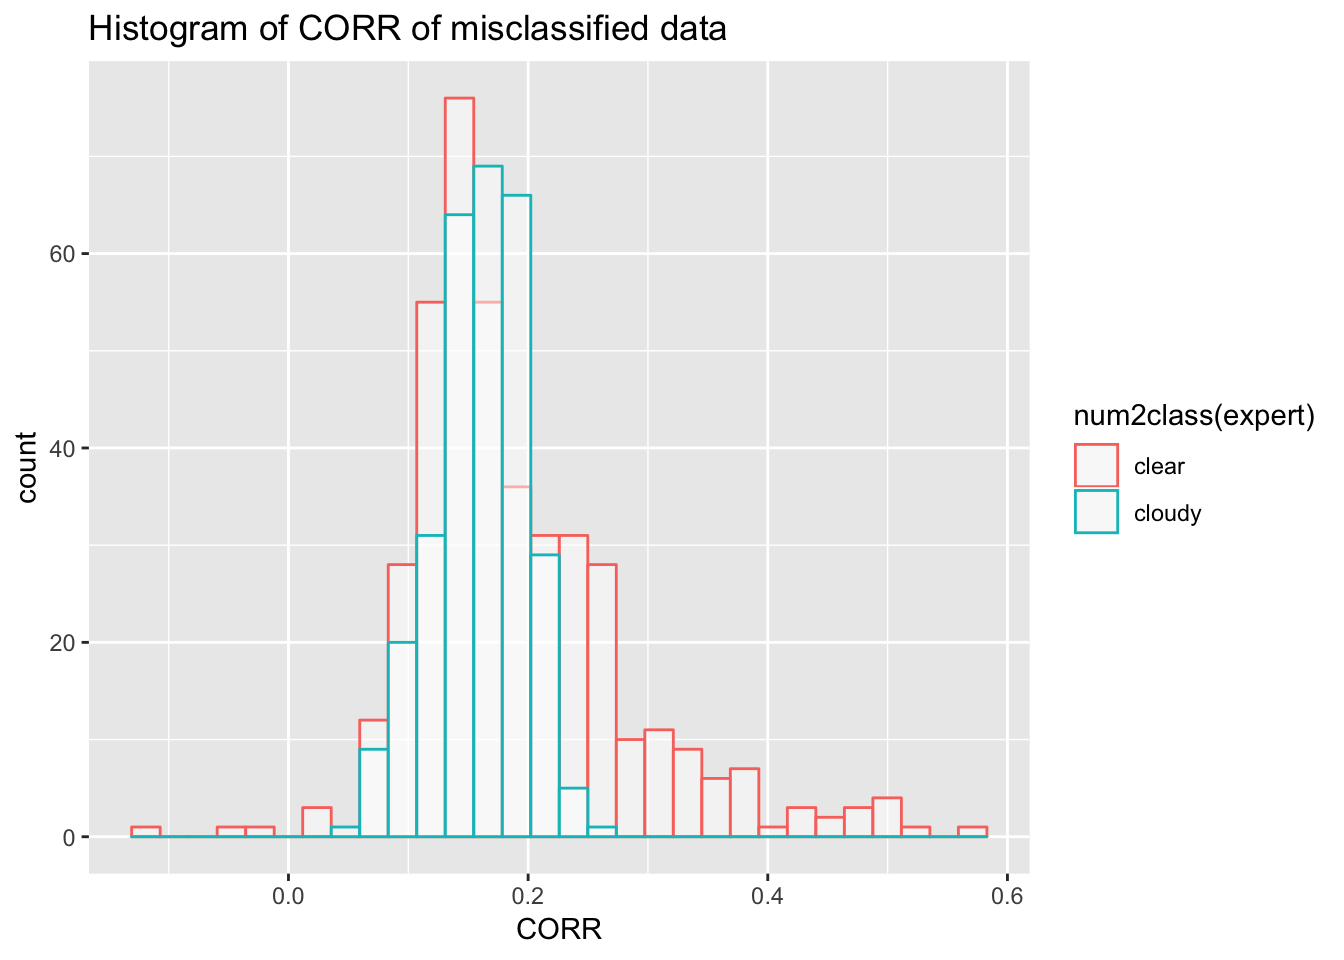
\includegraphics[scale=.1]{CORRmis}
    \caption{CORR}
    \label{fig:2}
  \end{subfigure}
 \caption{misclassified data}
\end{figure}

% \begin{figure*}[h]
% \begin{subfigure}{.4\textwidth}
% 	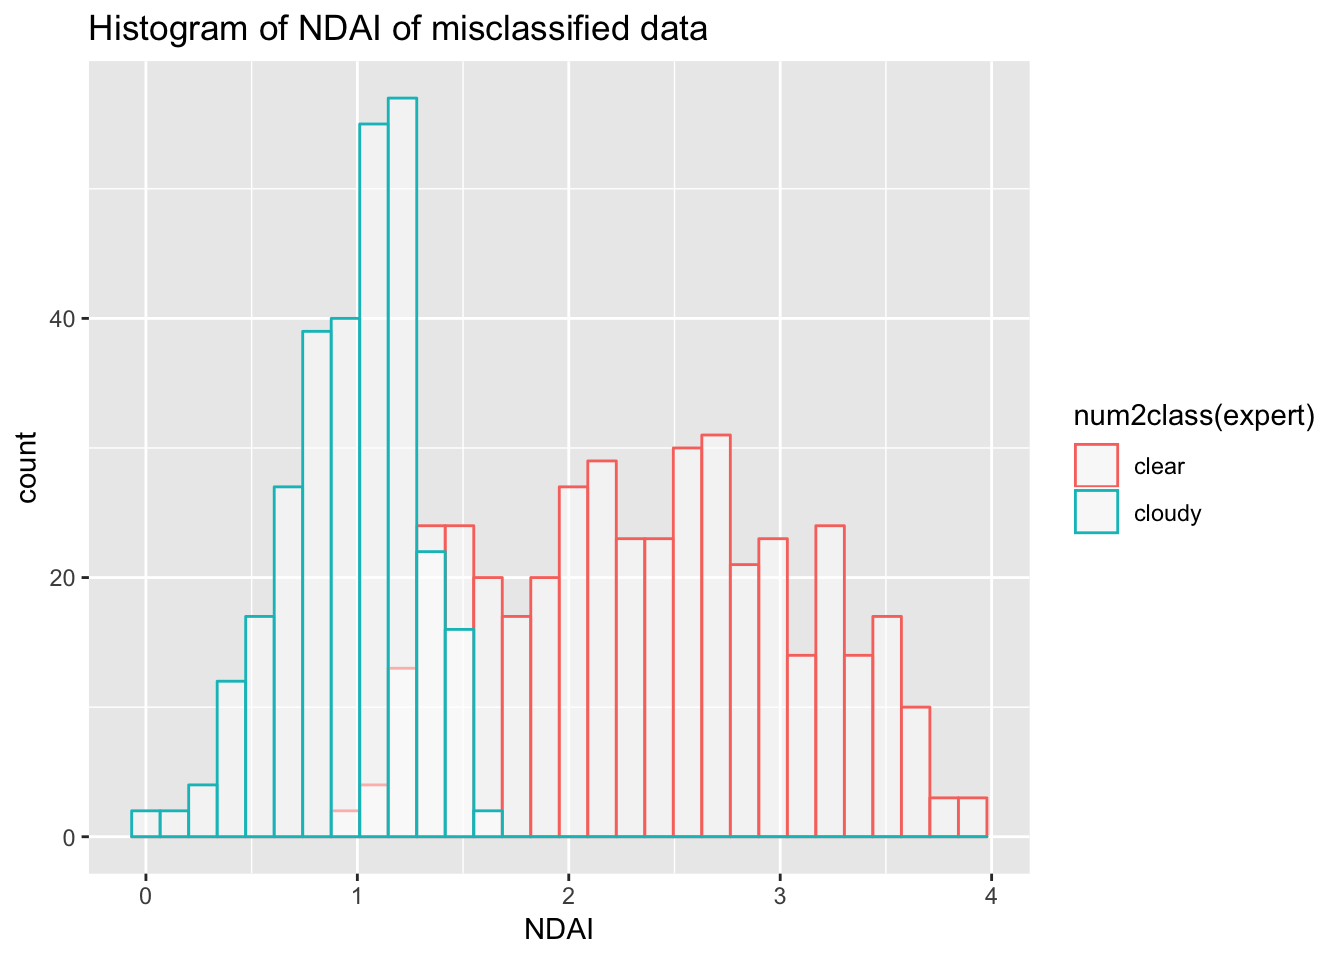
\includegraphics[scale=.1,]{NDAImis.png}
% 	\caption{NDAI}
% 	\label{fig:sub1}
% \end{subfigure}
% \begin{subfigure}{.4\textwidth}
% 	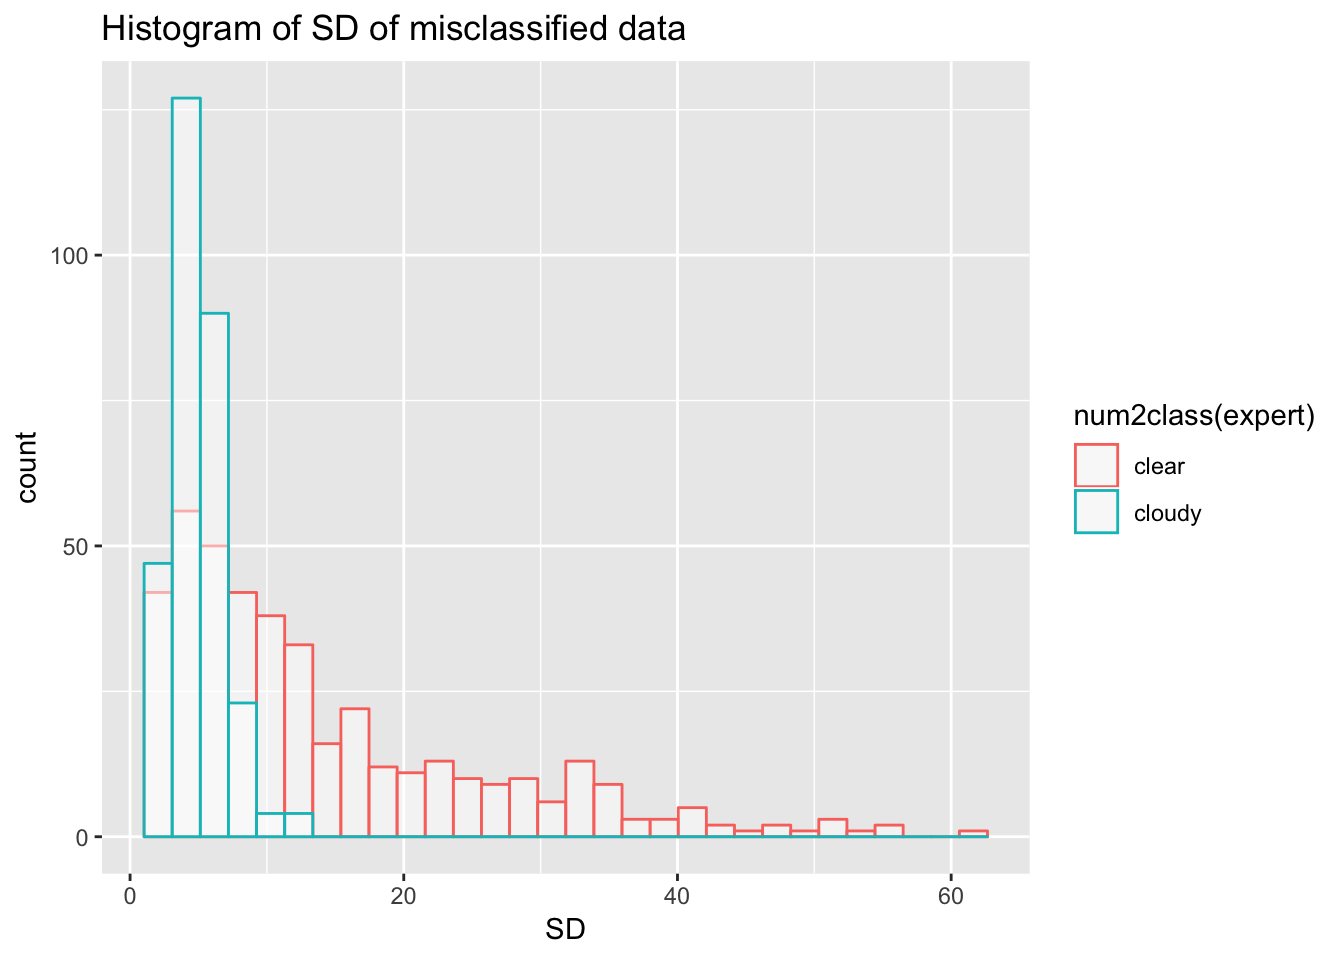
\includegraphics[scale=.1,]{SDmis.png}
% 	\caption{SD}
% 	\label{fig:sub2}
% \end{subfigure}
% \begin{subfigure}{.4\textwidth}
% 	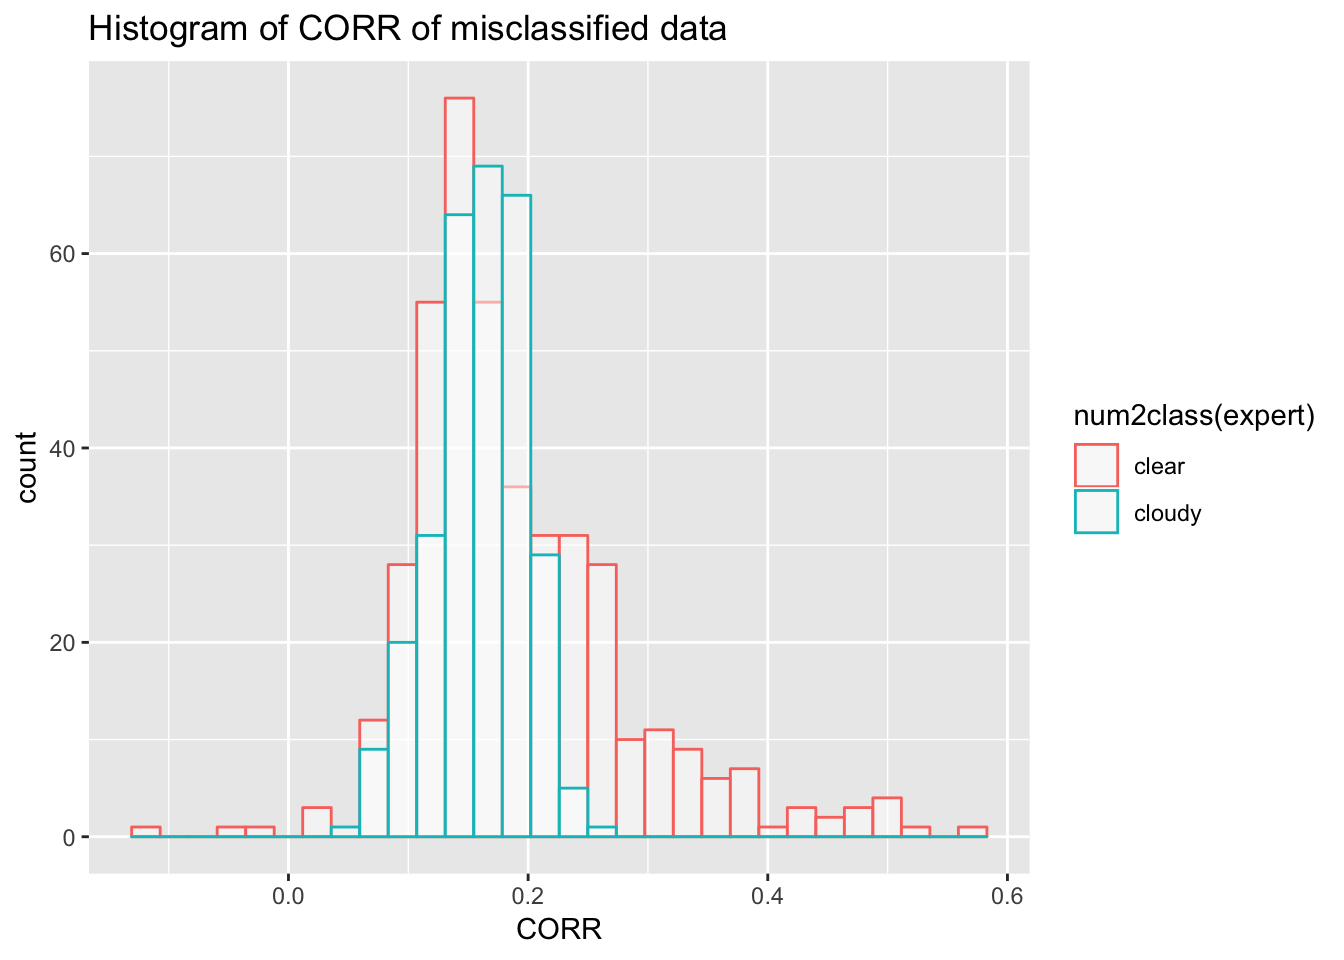
\includegraphics[scale=.1,]{CORRmis.png}
% 	\caption{CORR}
% 	\label{fig:sub3}
% \end{subfigure}
% \caption{misclassified data}
% \end{figure*}

The misclassified data distribution all have similar shape of the distribution in the original data. However, in the original distribution of all data (figure 5), cloudy areas on average have higher NDAI, SD, and CORR than clear areas on all data. (that is, the blue should be on the right side), but this graph of misclassified data shows the opposite. This makes sense because the misclassification usually happen when there is an anomaly in our feature. Our model expects cloudy region to have higher number in these feature so when this particular cloud's feature show the opposite, it is going to be misclassified. Now, let us take a look at the five radiance angles of the misclassified data:
\begin{figure}[H]\centering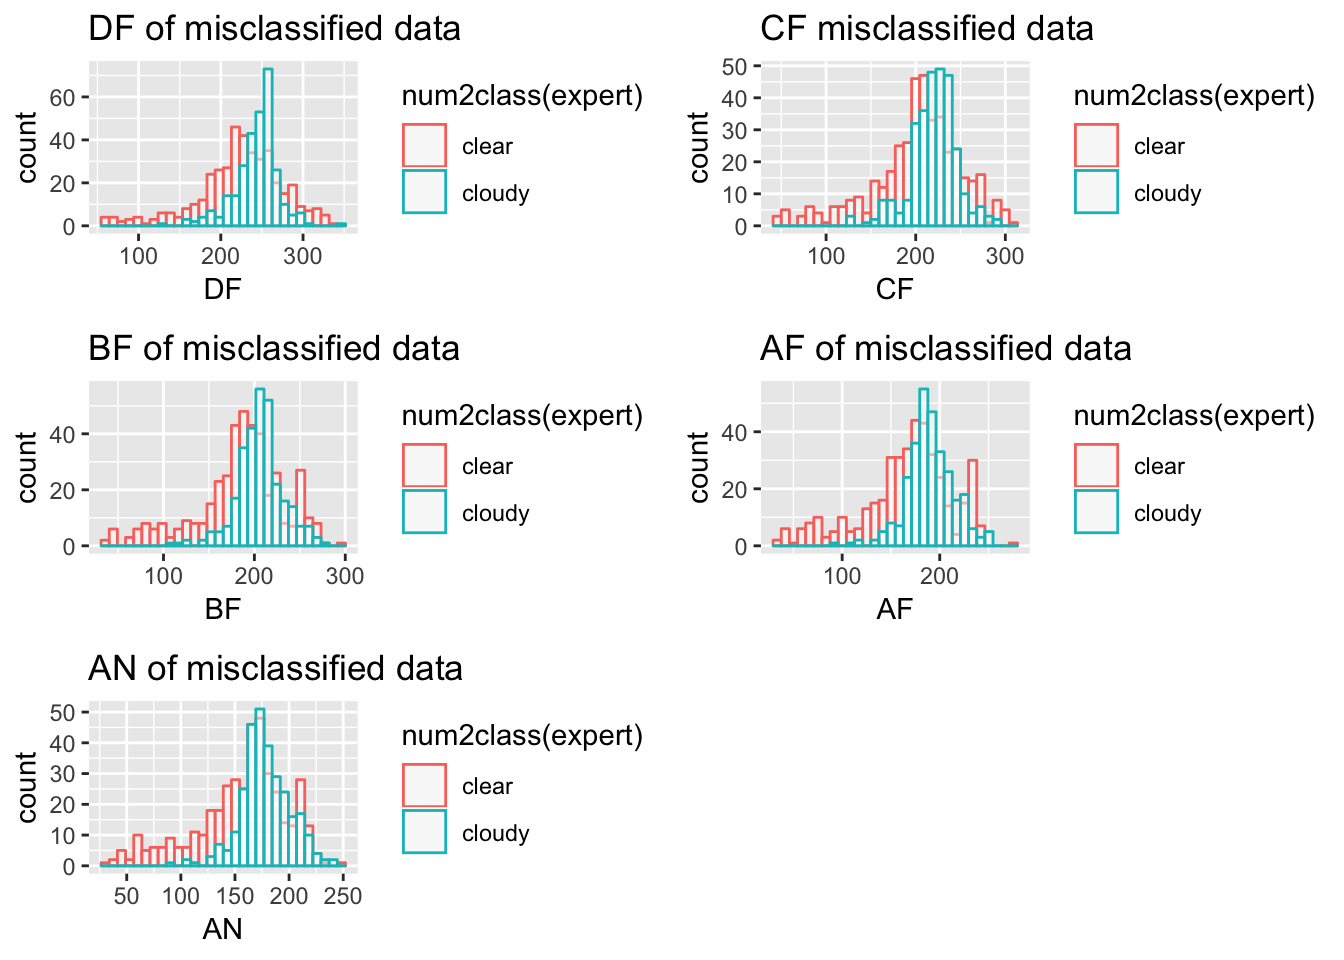
\includegraphics[scale=0.2,]{radiancemis}\vspace*{-0.5cm}\caption{Radiance Angle of misclassified data}\end{figure}
5 radiance readings show that the misclassified true clear data tend to be the ones with lower radiance readings. Before, we discussed that the radiance readings seem to be bi-modal. From the graph above, we can say that these misclassified data (whose true label is clear) seem to come from the left mode (one that is also lower). It seems that the  misclassified data seem to come from specific radiance reading range. It matches our previous observation that most of the misclassified data comes from image 3, which is shot from a particular radiance angle distinct from the other two images. It might be the case that the angles from which image 3 is shot is too noisy to be helpful to data classification.\\
\indent Now, let us poke further by plotting the misclassified data along with with feature distribution of the huge cloud in image 3 and of the entire cloudy data. As shown in figure 16 below, the blue distribution represents the distribution of the entire cloudy data, the red distribution represents the distribution of that big chunk of cloud in image 3, and the small green distribution represents the data that are false-clear, i.e., the data that is classified as clear but are actually cloud. For all of the three plots, the majority of the green lie inside of the red, meaning that most of the false-clear happen in the big cloud of image 3, matching what we found before. Additionally, we see that the red distribution is located to the left of the blue distribution, indicating that the big cloud in image 3 has NDAI, SD, and CORR lower than other clouds. Nonetheless, we observe that the misclassified data still have similar shape of distribution of feature as the non-misclassified data. 
\begin{figure}[H]
\hspace*{-.5cm}\begin{subfigure}{0.4\columnwidth}
    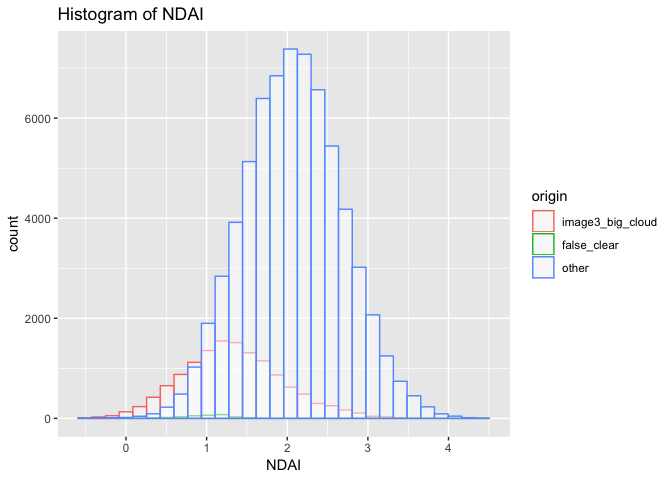
\includegraphics[scale=.2]{NDAIfalseclear}
    \caption{NDAI and image 3}
    \label{fig:1}
  \end{subfigure}\hfill %%
\begin{subfigure}{0.4\columnwidth} \hspace*{-1cm}
    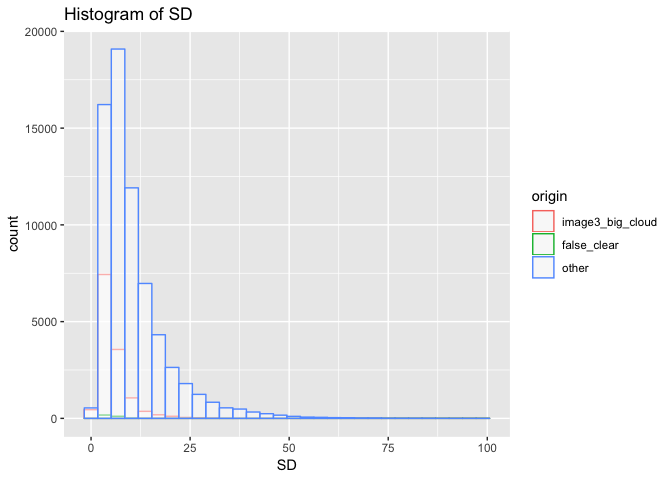
\includegraphics[scale=.2]{SDfalseclear}
    \caption{SD and image 3}
    \label{fig:2}
  \end{subfigure}
\hspace*{-.5cm}\begin{subfigure}{0.4\columnwidth}
    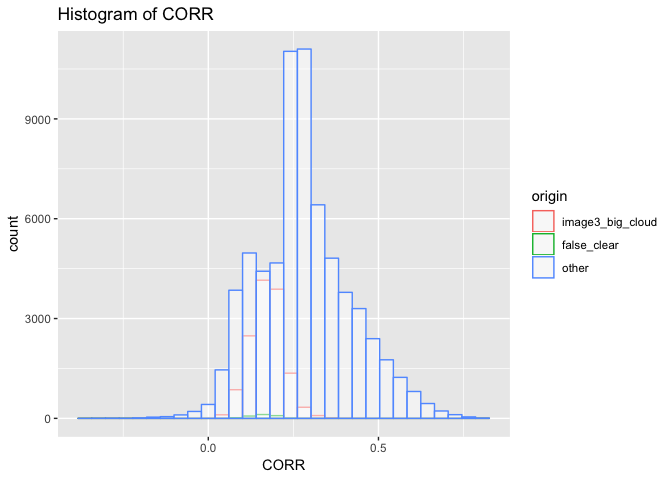
\includegraphics[scale=.2]{CORRfalseclear}
    \caption{CORR and image 3}
    \label{fig:2}
  \end{subfigure}
 \caption{features and image 3}
\end{figure}

\indent In sum the systematic error arises mainly because the huge chunk of cloud in image 3 has features that are systematically biased towards smaller values, perhaps as a result of inappropriate radiance angle in which image 3 was taken.

\subsection{c) Better Classifier}
To deal with the issue in b), we tried to modify the features and see if we can reduce the error. One way to modify the feature is to reduce their variance by reduce the differences between feature values of each data. By doing so, we hope that the abnormality in that big cloud can reduce as its feature value is closer to other clouds' so that the misclassification will be less pronounced. After tying a bunch of transformations, we decide to use the following. For each feature (NDAI, SD, CORR):
$$newfeature = log(feature - min(feature) + 1)$$
We first subtract the feature by the min so that the number inside the log is positive. We also add 1 so that the output of the log operation is also positive. Note that this is one choice of feature transformation that gives us a little improvement in our systematic classification error.\\
With the new features, we apply the same CV and classification method as part b) (i.e. image blurring and QDA) and we discover that the testing accuracy has improved by about 1\%:
\begin{verbatim}
##         old_model new_model
## 1         0.89733   0.91995
## 2         0.90339   0.91339
## 3         0.89928   0.91076
## 4         0.90373   0.91798
## 5         0.89823   0.91136
## 6         0.89969   0.90414
## 7         0.90095   0.91667
## 8         0.89879   0.92186
## 9         0.90004   0.89429
## 10        0.90109   0.90814
## -------   -------   -------
## average   0.90025   0.91185
\end{verbatim}
So this transformation looks promising. Also, it does not severely bias our misclassification error as before because the percentage of clear/cloudy data in the misclassified matches the percentage in the entire data:
\begin{verbatim}
##               clear    cloudy  
## misclassified "65.16%" "34.84%"
## total_labeled "61.08%" "38.92%"
\end{verbatim}
Under this new method, the systematic false cloudy error is reduced, although the total amount of the misclassified data did not change. The following graph is illustrative:
\begin{figure}[H]\hspace*{-2cm}\centering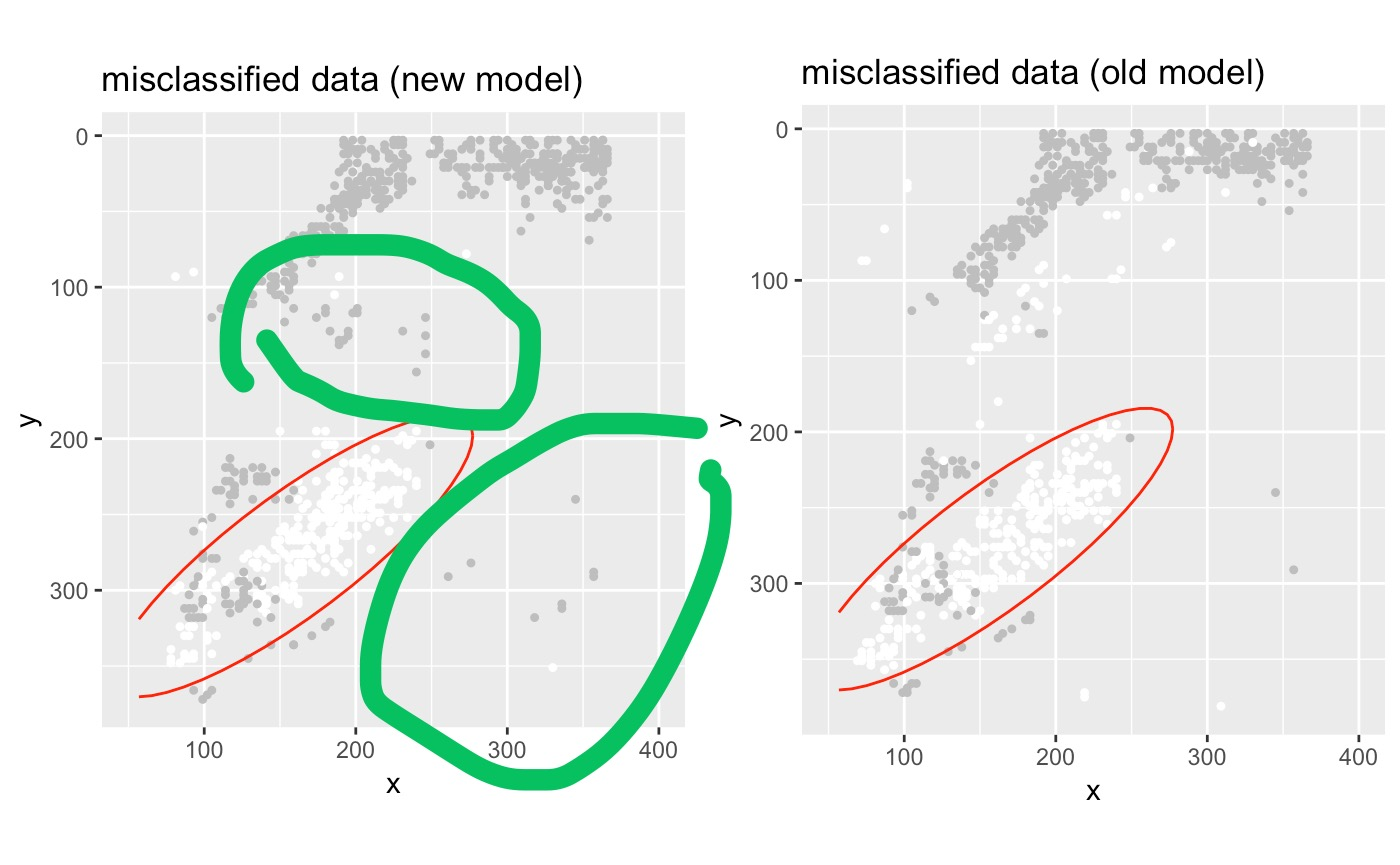
\includegraphics[width=8cm, height = 4cm]{newmis}\hspace*{-0.8cm}\caption{misclassified under new method}\end{figure}

Recall that the gray dots are false cloudy (clear region falsely classified as cloudy) and the white dots are false clear (cloudy region falsely classified as clear). Looking at the green circles, we find extra gray dots generated by the new model in regions where no gray dots are generated by the old model. After checking that the misclassification rates are the same between these two models, we can conclude that the systematic error of false cloudy has reduced because the gray dots are a little bit more spread out. Unfortunately, the new method does not help reducing the systematic error caused by the big cloud in image 3. We think our method will be good at classifying most of the future data. However, if the image in the data is shot from a similarly angle as image 3, our method might generate systematic error.


\subsection{d) Modification of Splitting}
Let us redo part a) and b) after splitting the data using \textbf{divide and sample}. First, we see a very different convergence trend of testing error:
\begin{figure}[H]\hspace*{-2cm} \centering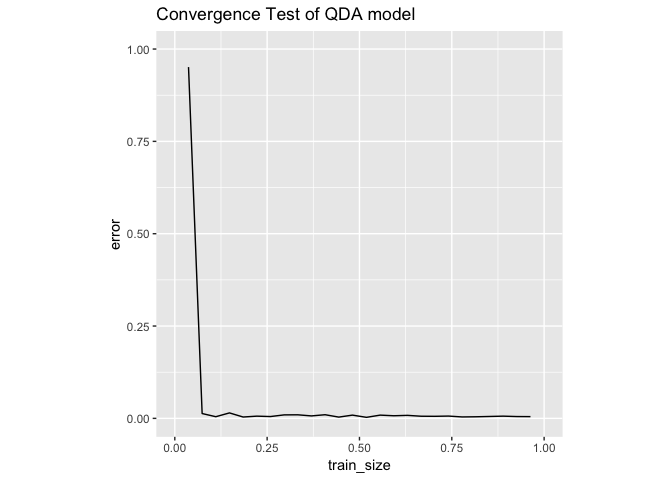
\includegraphics[width=12cm, height = 5cm]{convergeDivideSample}\caption{Error convergence according to divide and sample}\end{figure}
According to the divide and sample, it converges also very fast from getting everything wrong to getting most of the things right (error = 0). It converges when the training size is about 10\% of the entire data set. It differs from the image blurring method in that it converges a little bit slower because under the image blurring method, the error rate converges right away. However, it converges to a lower error rate than that of the image blurring method (10\% error rate) and after convergence, it is more stable or has less fluctuation. The reason is probably that the blurring method reduces the sample size to 10\% , which means that the divide and sample method has ten times the data size to train. If considering only 10\% of the training data set, image blurring method is not bad at all. The upshot is, according both splitting methods, QDA testing error converges quickly as the training size increases.\\
\indent After diagnosis, we take a look at the misclassified data. First, we notice a problem that the misclassified data is biased:
\begin{verbatim}
##               clear    cloudy  
## misclassified "75.85%" "24.15%"
## total_labeled "61.08%" "38.92%"
\end{verbatim} 
We observe that class percentage of misclassified data is different than the total class percentage. The model tends to misclassify clear regions as clouds more than vice versa. The testing error also goes up from 9.3332\% to 14.6620\% (after switching data splitting method from image blurring to divide and sample). Hence we can conclude that after changing splitting method, QDA is biased towards producing more false clear error and the QDA produces more testing errors. Plotted as images, the misclassified data also seem to cluster around, indicating a systematic error under this splitting method:
\begin{figure}[H] \centering\hspace*{-0.5cm} 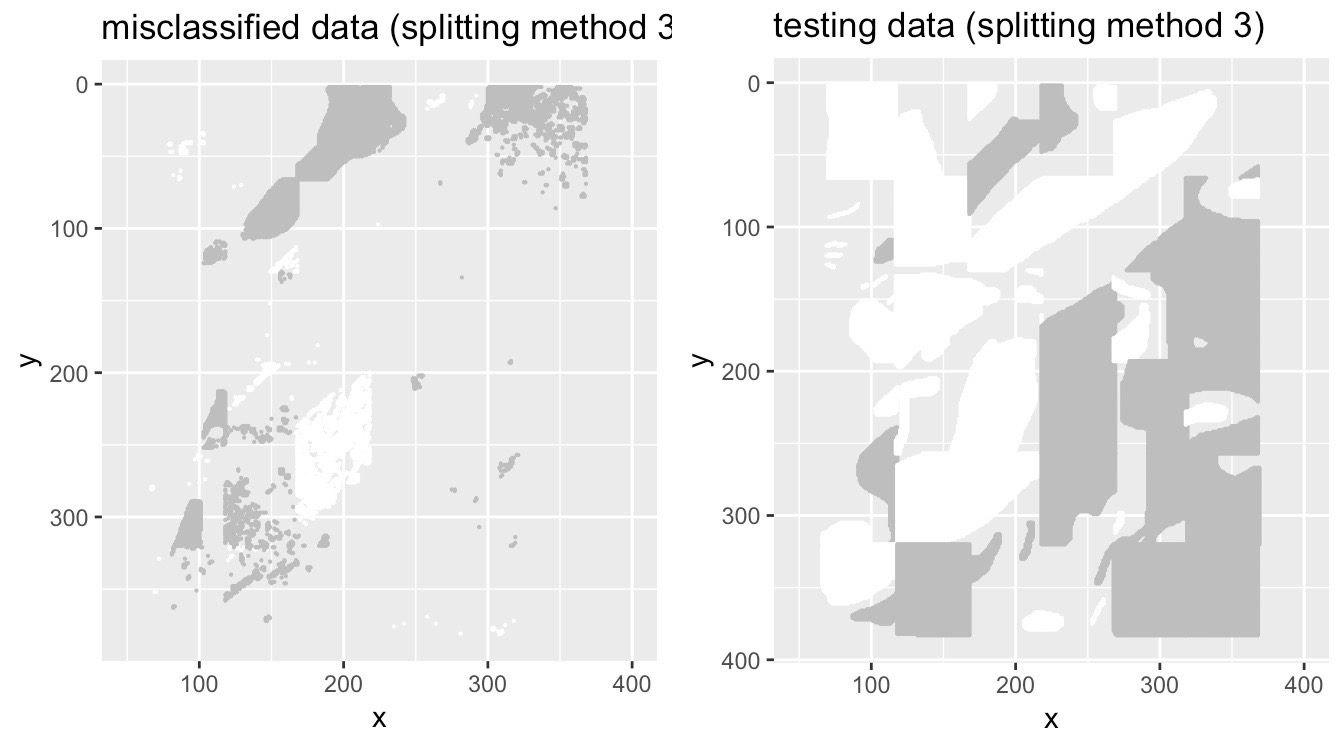
\includegraphics[width=9cm, height = 4cm]{splitmis}\vspace*{-0.2cm} \caption{misclassified under another splitting}\end{figure}
It is reasonable to suspect that the same systematic error still lingers as we can see the white region in the bottom left subimage of the "misclassified data" matches the location of the huge cloud in image 3, although it is fragmented. At the top of this image, the gray area also reveals a similar pattern as the one produced by the image blurring method. At the first glance, it does not seem that a change in splitting method can help and the systematic error may be attributed to the classification method. However, let us take a closer look at the features:

\begin{figure}[H]
\hspace*{-.5cm}\begin{subfigure}{0.4\columnwidth}
    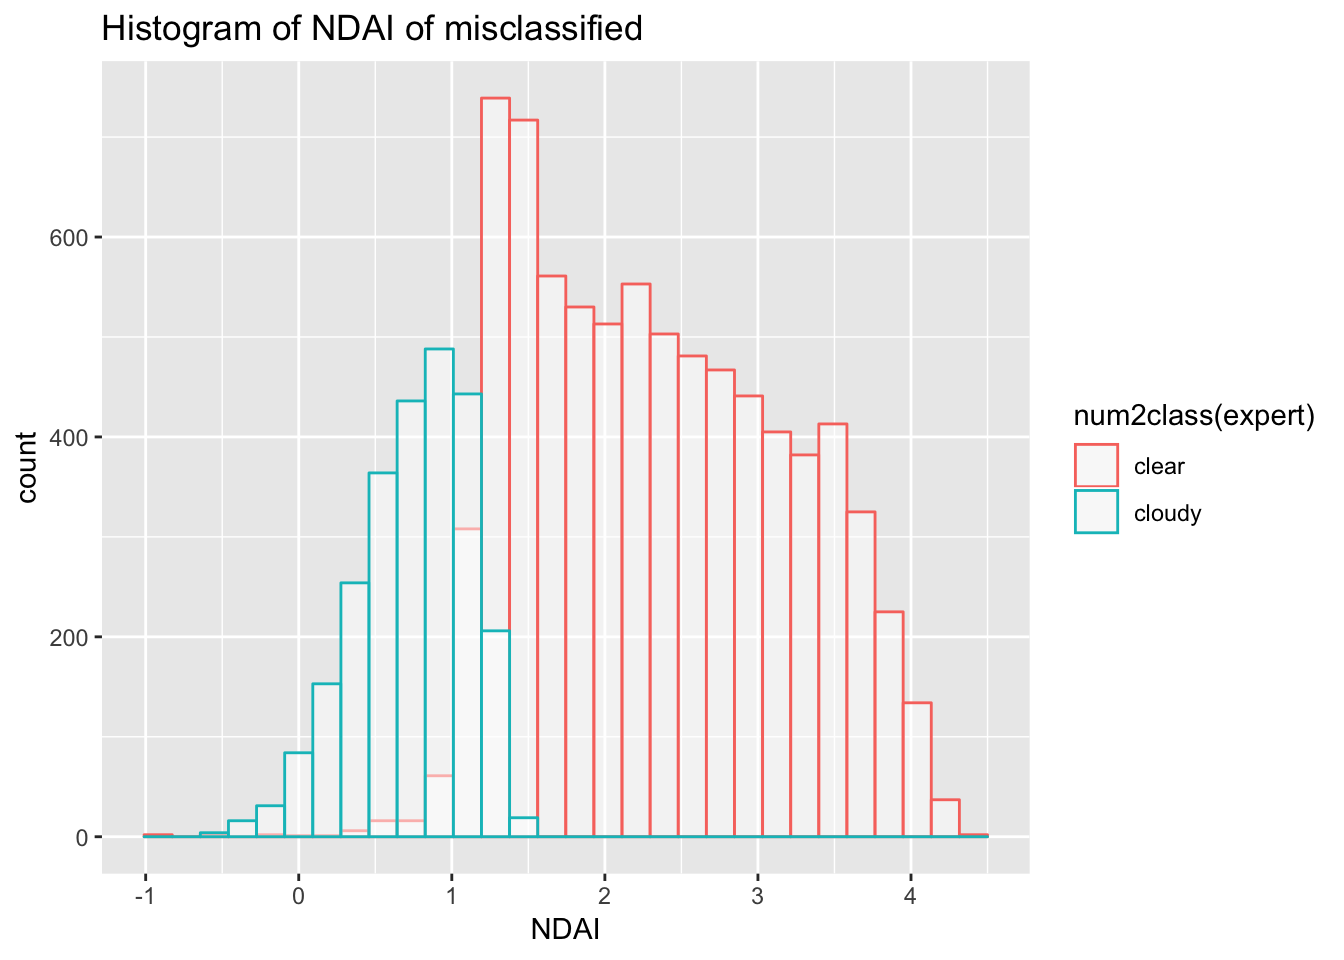
\includegraphics[scale=.1]{NDAIsplit}
    \caption{NDAI}
    \label{fig:1}
  \end{subfigure}\hfill %%
\begin{subfigure}{0.4\columnwidth} \hspace*{-1cm}
    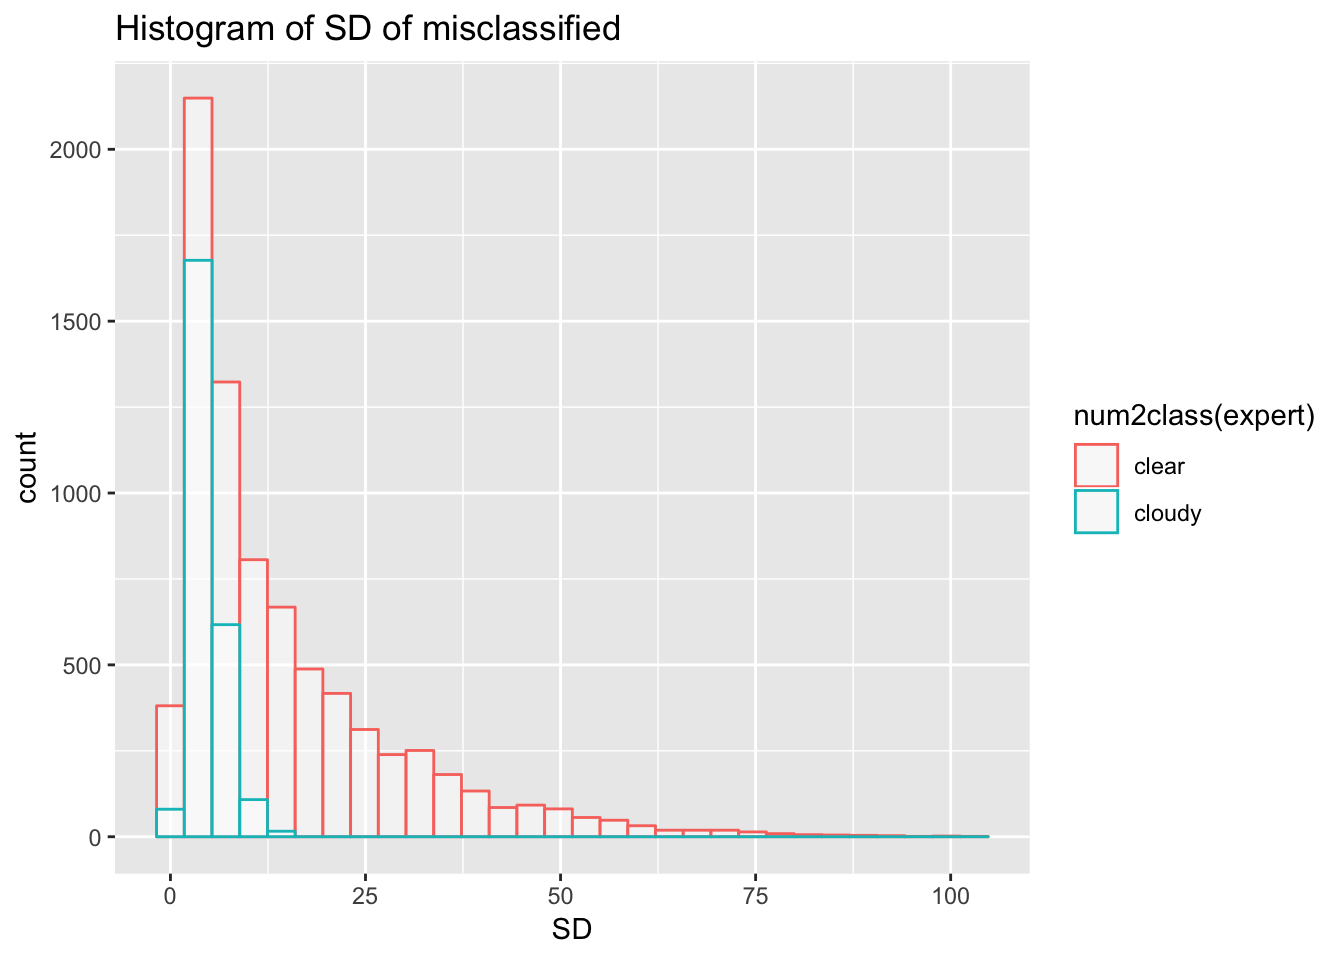
\includegraphics[scale=.1]{SDsplit}
    \caption{SD}
    \label{fig:2}
  \end{subfigure}
\hspace*{-.5cm}\begin{subfigure}{0.4\columnwidth}
    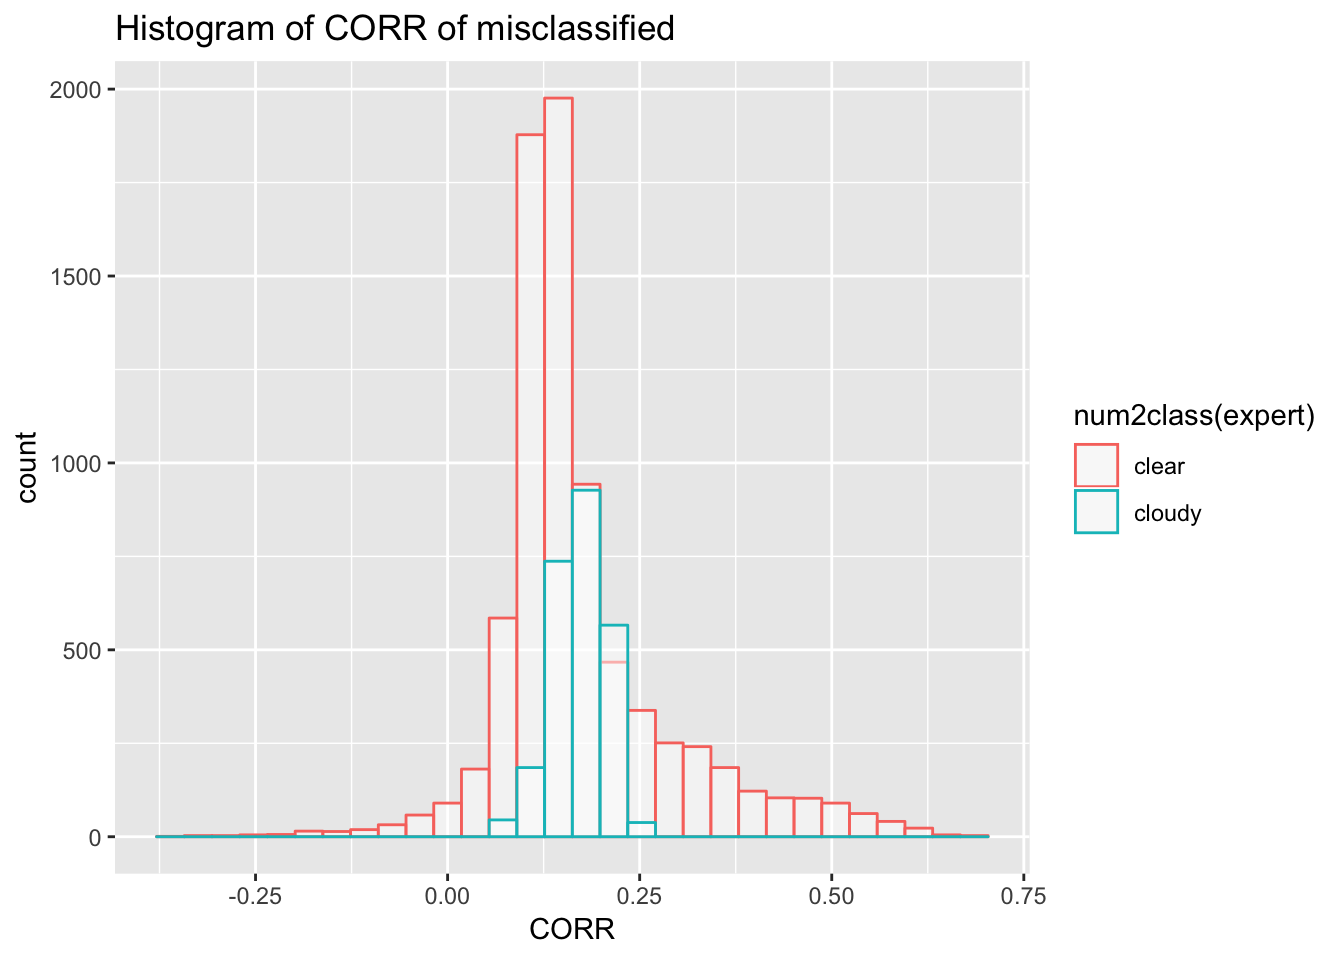
\includegraphics[scale=.1]{CORRsplit}
    \caption{CORR}
    \label{fig:2}
  \end{subfigure}
 \caption{misclassified with another split method}
\end{figure}

The general trend remains the same as our part b), although it is again clear that the misclassified data is biased towards classifying clear region into clouds because we have overall higher red columns in each histograms. This echoes our quantitative result resented before. We can also observe that the true cloudy regions being misclassified still have abnormally low values on NDAI and SD because the green distribution is center around the left side of the red distribution, but the deviation seems to be less pronounced for CORR. Nonetheless, when we look at the quantitative result of the number of standard deviation from the mean, we are more assured that a change of splitting method does not significantly reduce the systematic error:
\begin{verbatim}
##      false clear false cloudy
## NDAI  -1.7906904sd    2.4588215sd
## SD    -0.6318481sd    1.9695497sd
## CORR  -0.6898196sd    0.6936461sd
\end{verbatim}
As we can see, the deviation of feature values are just as large as when we use image blurring method, with only some decrease in CORR value under false cloudy, which matches our graphical observation in the histogram above. Lastly, let us take a look at the radiance angle:
\begin{figure}[H] \centering\hspace*{-0.5cm}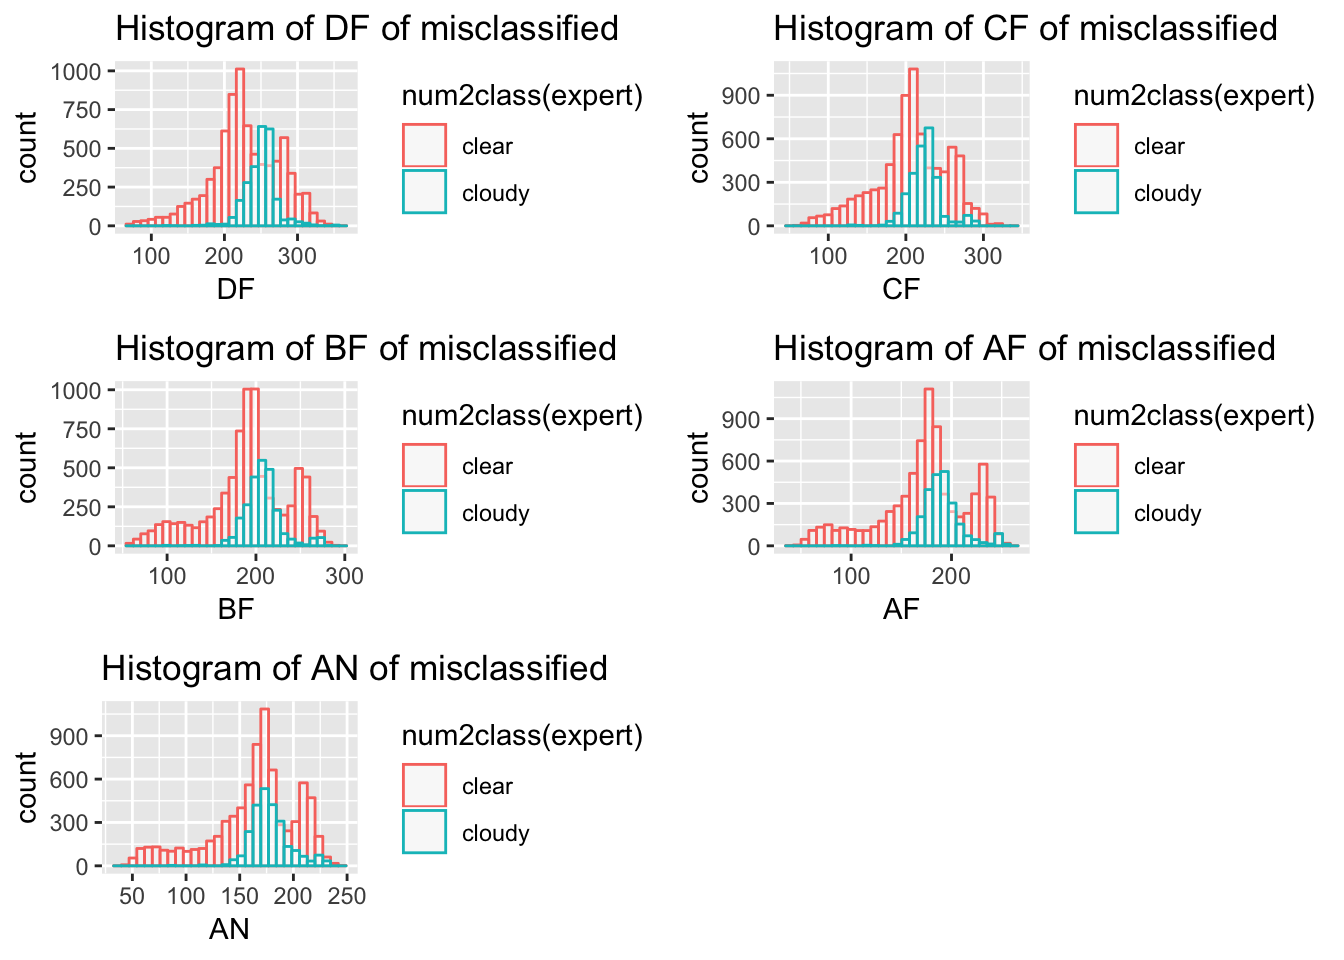
\includegraphics[scale=0.2,]{radiancesplit}\caption{Radiance Angle of misclassified data}\end{figure}
Here we discover something informative. Recall in the previous part, we found out that 5 radiance readings show that the misclassified true clear data tend to be the ones with lower radiance readings because the misclassified clear region form a uni-modal distribution instead of the bi-modal one in our original data. From the graph above, we are surprised that the bimodal pattern has returned. This shows that this way of splitting data creates additional systematic error in the high radiance data as well. In sum, changing the data splitting method does not seem to help much. It reduces the error in CORR a little, but introduces extra systematic error in the radiance angles.

\subsection{e) Conclusion}
In the project, we first explored the domain question and the data involved in Prof. Yu's paper and decided to focus on NDAI, SD, and CORR as the main features to classify the cloud regions from the clear regions in meterological photographs taken from the space. Then for cross validation, We explored three ways to split the data which is not independent: divide and sample, divide and forge, and image blurring. We discovered that image blurring outperforms other methods and thus we selected it as the main method for performing cross validation. After cross validation, we considered four classification methods: LDA, QDA, logistic regression, and decision tree. We attempted SVM and adaboost but unfortunately, the are too computationally expensive even though they might yield better fitting. To select the methods, we used the ROC curve and QDA excels slightly. We end up have a testing accuracy of about 91\%.\\
\indent Based upon QDA and image blurring method, we dig deeper into the systematic misclassification lurking behind. We discovered that most of the systematic errors come from a huge cloud in image 3 where the feature values are unusually low. We suspect that the reason is that image 3 is shot from an awkward radiance angle so that the data collected is too noisy for our classification methods. We attempted at transforming the three features with a log based function and the systematic classification error only reduced very sightly. We also tried to change the data splitting method and no significant improvement was detected either. More work need to be done in eliminating the systematic error. To do so, one might have to classify data separately.\\


github link: \href{https://github.com/hutou2014/stat154_proj2}{$https://github.com/hutou2014/stat154\_proj2$}

\begin{table}[h]
\caption{Acknowledgment (P = Ham, D = Xuanfu):}
\label{tab:tab1}
\begin{tabular}{|cccc|}\hline
Parts  & Solving  & Coding & Writing \\ \hline
1(a)     & P    & NA & P \\
1(b)     &    D       &    D     & P \\
1(c)    & D    & D   & P \\
2(a)         &    D+P      &    D+P      & P \\ 
2(b)    & D+P    & D   & P \\
2(c)    & D+P    & P   & P \\
2(d)    & D    & D   & NA \\
3(a)    & D+P    & D+P   & P \\
3(b)    & D+P    & D+P   & P \\
3(c)    & D+P    & D+P   & P \\
4(a)    & P    & D   & P \\
4(b)    & D    & D   & P \\
4(c)    & D+P    & D   & P \\
4(d)    & D    & D   & P \\
4(e)    & P    & NA   & P \\
5       & D+P    & D   & P \\\hline
\end{tabular}
\end{table}  


\end{document}